% Options for packages loaded elsewhere
\PassOptionsToPackage{unicode}{hyperref}
\PassOptionsToPackage{hyphens}{url}
\PassOptionsToPackage{dvipsnames,svgnames*,x11names*}{xcolor}
%
\documentclass[
  12pt,
]{book}
\usepackage{amsmath,amssymb}
\usepackage{lmodern}
\usepackage{setspace}
\usepackage{ifxetex,ifluatex}
\ifnum 0\ifxetex 1\fi\ifluatex 1\fi=0 % if pdftex
  \usepackage[T1]{fontenc}
  \usepackage[utf8]{inputenc}
  \usepackage{textcomp} % provide euro and other symbols
\else % if luatex or xetex
  \usepackage{unicode-math}
  \defaultfontfeatures{Scale=MatchLowercase}
  \defaultfontfeatures[\rmfamily]{Ligatures=TeX,Scale=1}
\fi
% Use upquote if available, for straight quotes in verbatim environments
\IfFileExists{upquote.sty}{\usepackage{upquote}}{}
\IfFileExists{microtype.sty}{% use microtype if available
  \usepackage[]{microtype}
  \UseMicrotypeSet[protrusion]{basicmath} % disable protrusion for tt fonts
}{}
\makeatletter
\@ifundefined{KOMAClassName}{% if non-KOMA class
  \IfFileExists{parskip.sty}{%
    \usepackage{parskip}
  }{% else
    \setlength{\parindent}{0pt}
    \setlength{\parskip}{6pt plus 2pt minus 1pt}}
}{% if KOMA class
  \KOMAoptions{parskip=half}}
\makeatother
\usepackage{xcolor}
\IfFileExists{xurl.sty}{\usepackage{xurl}}{} % add URL line breaks if available
\IfFileExists{bookmark.sty}{\usepackage{bookmark}}{\usepackage{hyperref}}
\hypersetup{
  pdftitle={Software implementations allowing new approaches toward data analysis, modeling and curation of biological knowledge for Systems Medicine},
  pdfauthor={John Zobolas},
  colorlinks=true,
  linkcolor=blue,
  filecolor=Maroon,
  citecolor=Blue,
  urlcolor=blue,
  pdfcreator={LaTeX via pandoc}}
\urlstyle{same} % disable monospaced font for URLs
\usepackage[left=2.5cm, right=2.5cm, top=2.5cm, bottom=2.5cm]{geometry}
\usepackage{longtable,booktabs,array}
\usepackage{calc} % for calculating minipage widths
% Correct order of tables after \paragraph or \subparagraph
\usepackage{etoolbox}
\makeatletter
\patchcmd\longtable{\par}{\if@noskipsec\mbox{}\fi\par}{}{}
\makeatother
% Allow footnotes in longtable head/foot
\IfFileExists{footnotehyper.sty}{\usepackage{footnotehyper}}{\usepackage{footnote}}
\makesavenoteenv{longtable}
\usepackage{graphicx}
\makeatletter
\def\maxwidth{\ifdim\Gin@nat@width>\linewidth\linewidth\else\Gin@nat@width\fi}
\def\maxheight{\ifdim\Gin@nat@height>\textheight\textheight\else\Gin@nat@height\fi}
\makeatother
% Scale images if necessary, so that they will not overflow the page
% margins by default, and it is still possible to overwrite the defaults
% using explicit options in \includegraphics[width, height, ...]{}
\setkeys{Gin}{width=\maxwidth,height=\maxheight,keepaspectratio}
% Set default figure placement to htbp
\makeatletter
\def\fps@figure{htbp}
\makeatother
\setlength{\emergencystretch}{3em} % prevent overfull lines
\providecommand{\tightlist}{%
  \setlength{\itemsep}{0pt}\setlength{\parskip}{0pt}}
\setcounter{secnumdepth}{5}
% for figures to fit (sometimes works well)
%\renewcommand{\textfraction}{0.05}
%\renewcommand{\topfraction}{0.8}
%\renewcommand{\bottomfraction}{0.8}
%\renewcommand{\floatpagefraction}{0.75}

% removes section headings from the top of pages
\pagestyle{plain}

\usepackage{color}
\usepackage{xcolor}
\usepackage{framed}
\usepackage{tcolorbox}
\usepackage{pdfpages}

% define color boxes
\setlength{\fboxsep}{.8em}

\newenvironment{blackbox}{
  \definecolor{shadecolor}{rgb}{0, 0, 0}  % black
  \color{white}
  \begin{shaded}}
 {\end{shaded}}

\definecolor{lightblue}{HTML}{E6F0FF}

\newtcolorbox{blue-box}{
  colback=lightblue,
  colframe=white,
  coltext=black,
  boxsep=5pt,
  arc=4pt}

% to right align
\newenvironment{right-align}{
  \begin{flushright}}
 {\end{flushright}}

% Nice font styleing for pdf text
\usepackage{type1cm}
%% Replace the standard Computer Modern Typewriter font LaTeX uses
%% for monospace text with the PostScript font Adobe Courier.
%\usepackage{courier}
\usepackage[T1]{fontenc}
\usepackage[utf8]{inputenc}
\usepackage{ae,aecompl}
\usepackage{times}
%% Redefine the font used for the section headings to
%% Helvetica-Narrow Bold.
\usepackage{sectsty}
\allsectionsfont{\usefont{OT1}{phv}{bc}{n}\selectfont}

% reduce figure caption size
\usepackage{caption}
\captionsetup[figure]{font=footnotesize}

% for multiple-page, better-looking abbreviations table
\usepackage{longtable}
\usepackage{booktabs}

% for numbering
\frontmatter
\ifluatex
  \usepackage{selnolig}  % disable illegal ligatures
\fi
\newlength{\cslhangindent}
\setlength{\cslhangindent}{1.5em}
\newlength{\csllabelwidth}
\setlength{\csllabelwidth}{3em}
\newenvironment{CSLReferences}[2] % #1 hanging-ident, #2 entry spacing
 {% don't indent paragraphs
  \setlength{\parindent}{0pt}
  % turn on hanging indent if param 1 is 1
  \ifodd #1 \everypar{\setlength{\hangindent}{\cslhangindent}}\ignorespaces\fi
  % set entry spacing
  \ifnum #2 > 0
  \setlength{\parskip}{#2\baselineskip}
  \fi
 }%
 {}
\usepackage{calc}
\newcommand{\CSLBlock}[1]{#1\hfill\break}
\newcommand{\CSLLeftMargin}[1]{\parbox[t]{\csllabelwidth}{#1}}
\newcommand{\CSLRightInline}[1]{\parbox[t]{\linewidth - \csllabelwidth}{#1}\break}
\newcommand{\CSLIndent}[1]{\hspace{\cslhangindent}#1}

\title{Software implementations allowing new approaches toward data analysis, modeling and curation of biological knowledge for Systems Medicine}
\usepackage{etoolbox}
\makeatletter
\providecommand{\subtitle}[1]{% add subtitle to \maketitle
  \apptocmd{\@title}{\par {\large #1 \par}}{}{}
}
\makeatother
\subtitle{~\\
Doctoral thesis\\
\hspace*{0.333em}\\
Norwegian University of Science and Technology\\
Faculty of Natural Sciences\\
Department of Biology}
\author{John Zobolas}
\date{Trondheim, May 2021}

\begin{document}
\maketitle

{
\hypersetup{linkcolor=}
\setcounter{tocdepth}{1}
\tableofcontents
}
\setstretch{1.2}
\hypertarget{acknowledgements}{%
\chapter*{Acknowledgements}\label{acknowledgements}}
\addcontentsline{toc}{chapter}{Acknowledgements}

I first acknowledge funding from the \textbf{ERACoSysMed project COLOSYS}. Now to people, the most important part: \textbf{I would like to thank everyone} that interacted with me during the years I conducted my PhD research (2017-2021), even for a tiny bit. A person is only a small node in a complex network of interactions, which only when considered together, make up the person. In other words, you are not just you! So, you were \textbf{all important} for me (and for others I am sure)! Importance though is measured in varying degrees. Therefore now, I will proceed to give some personal credits (the part that most of you came here to read :)

A big \textbf{THANK YOU} to my supervisor, Prof.~Martin Kuiper. He gave me the opportunity to come to Norway, which opened a world of possibilities. The dream supervisor everyone should have and a caring human being above all. A true gentleman and an unsurpassed cook as well!

To Dr.~Åsmund Flobak for excellent co-supervision, the nice scientific discussions we had and for introducing me into \texttt{R}, which largely influenced the way I do science. Spending time with his lively family was always a nice change of pace. That day we were all together at Amsterdam's zoo and I saw my first penguins, will remain unforgettable!

To Dr.~Steven Vercruysse for our scientific discussions and for teaching me and ins and outs of web software development. I will never forget the ELIXIR Biohackathon 2020, great laughs and great work, all in one. And of course, I will never forget the ``tour'' . Thanks Steven!

To Prof.~Astrid Laegreid, for suggesting to me to participate in the Responsible Research and Innovation (RRI) course, which inspired me to think more broadly about my research and the world we live in, and of course meet several wonderful people! That's also how I became acquainted with Digital Life Norway (DLN). Liv Eggset Falkenberg did an excellent job at coordinating the DLN Research School and she was co-organizer of the Walkshop in Jotunheimen (September 2019), which was a truly wonderful experience. With DLN, I had the benefit of participating in various conferences across Norway and the opportunity to do an industry internship in Sweden during the cold winter of 2021, so thanks DLN and Liv!

To Noemi Del Toro Ayllon, for introducing me to the professional world of software development and project management with Java. Visiting the IntAct team at EBI during the summer of 2018 was a memorable experience and when she came to Trondheim later in 2019, we had such a great time, so thank you Noe!

To Henning Hermjacob, for not just being the scientific host for my visits to EBI in England, but also for hosting me in his lovely Airbnb house each time! Spending a few months in Cambridge during my PhD was a truly marvelous experience, so thanks Henning!

To Prof.~Denis Thieffry, for the nice scientific discussions and for distilling some of his passion for logical modeling into me, resulting in one of the papers in this thesis.

And of course, \textbf{to my colleagues from the DrugLogics group}, for the good times we spent inside and outside of work! I am especially grateful to Barbara Niederdorfer and Evelina Folkesson for our music collaborations. Eirini Tsirvouli has been a very positive, dynamic presence. Rafel Riudavets Puig has been a really close friend - I hope that in the future we get to continue our random walks that somehow always end up in McDonalds! Marcio Luis Acencio has been a good friend as well, with a wonderful family that gained two new members I got to meet before he left our group! Vasundra Touré has been a wonderful colleague, a true source of light for the time we spend at our office in Gloshaugen. Wine, cheese, standards and good memories! Also, favorite cafe buddies with Anamika Chatterjee - we certainly made Espresso House richer!

Last but not least, a big \textbf{THANKS} to the beautiful city of Trondheim! I've had some really inspirational walks in these historic roads. And to its nice coffee shops I've been working throughout my PhD! Diverse working environment is extremely important and as it was perfectly stated:

\begin{center}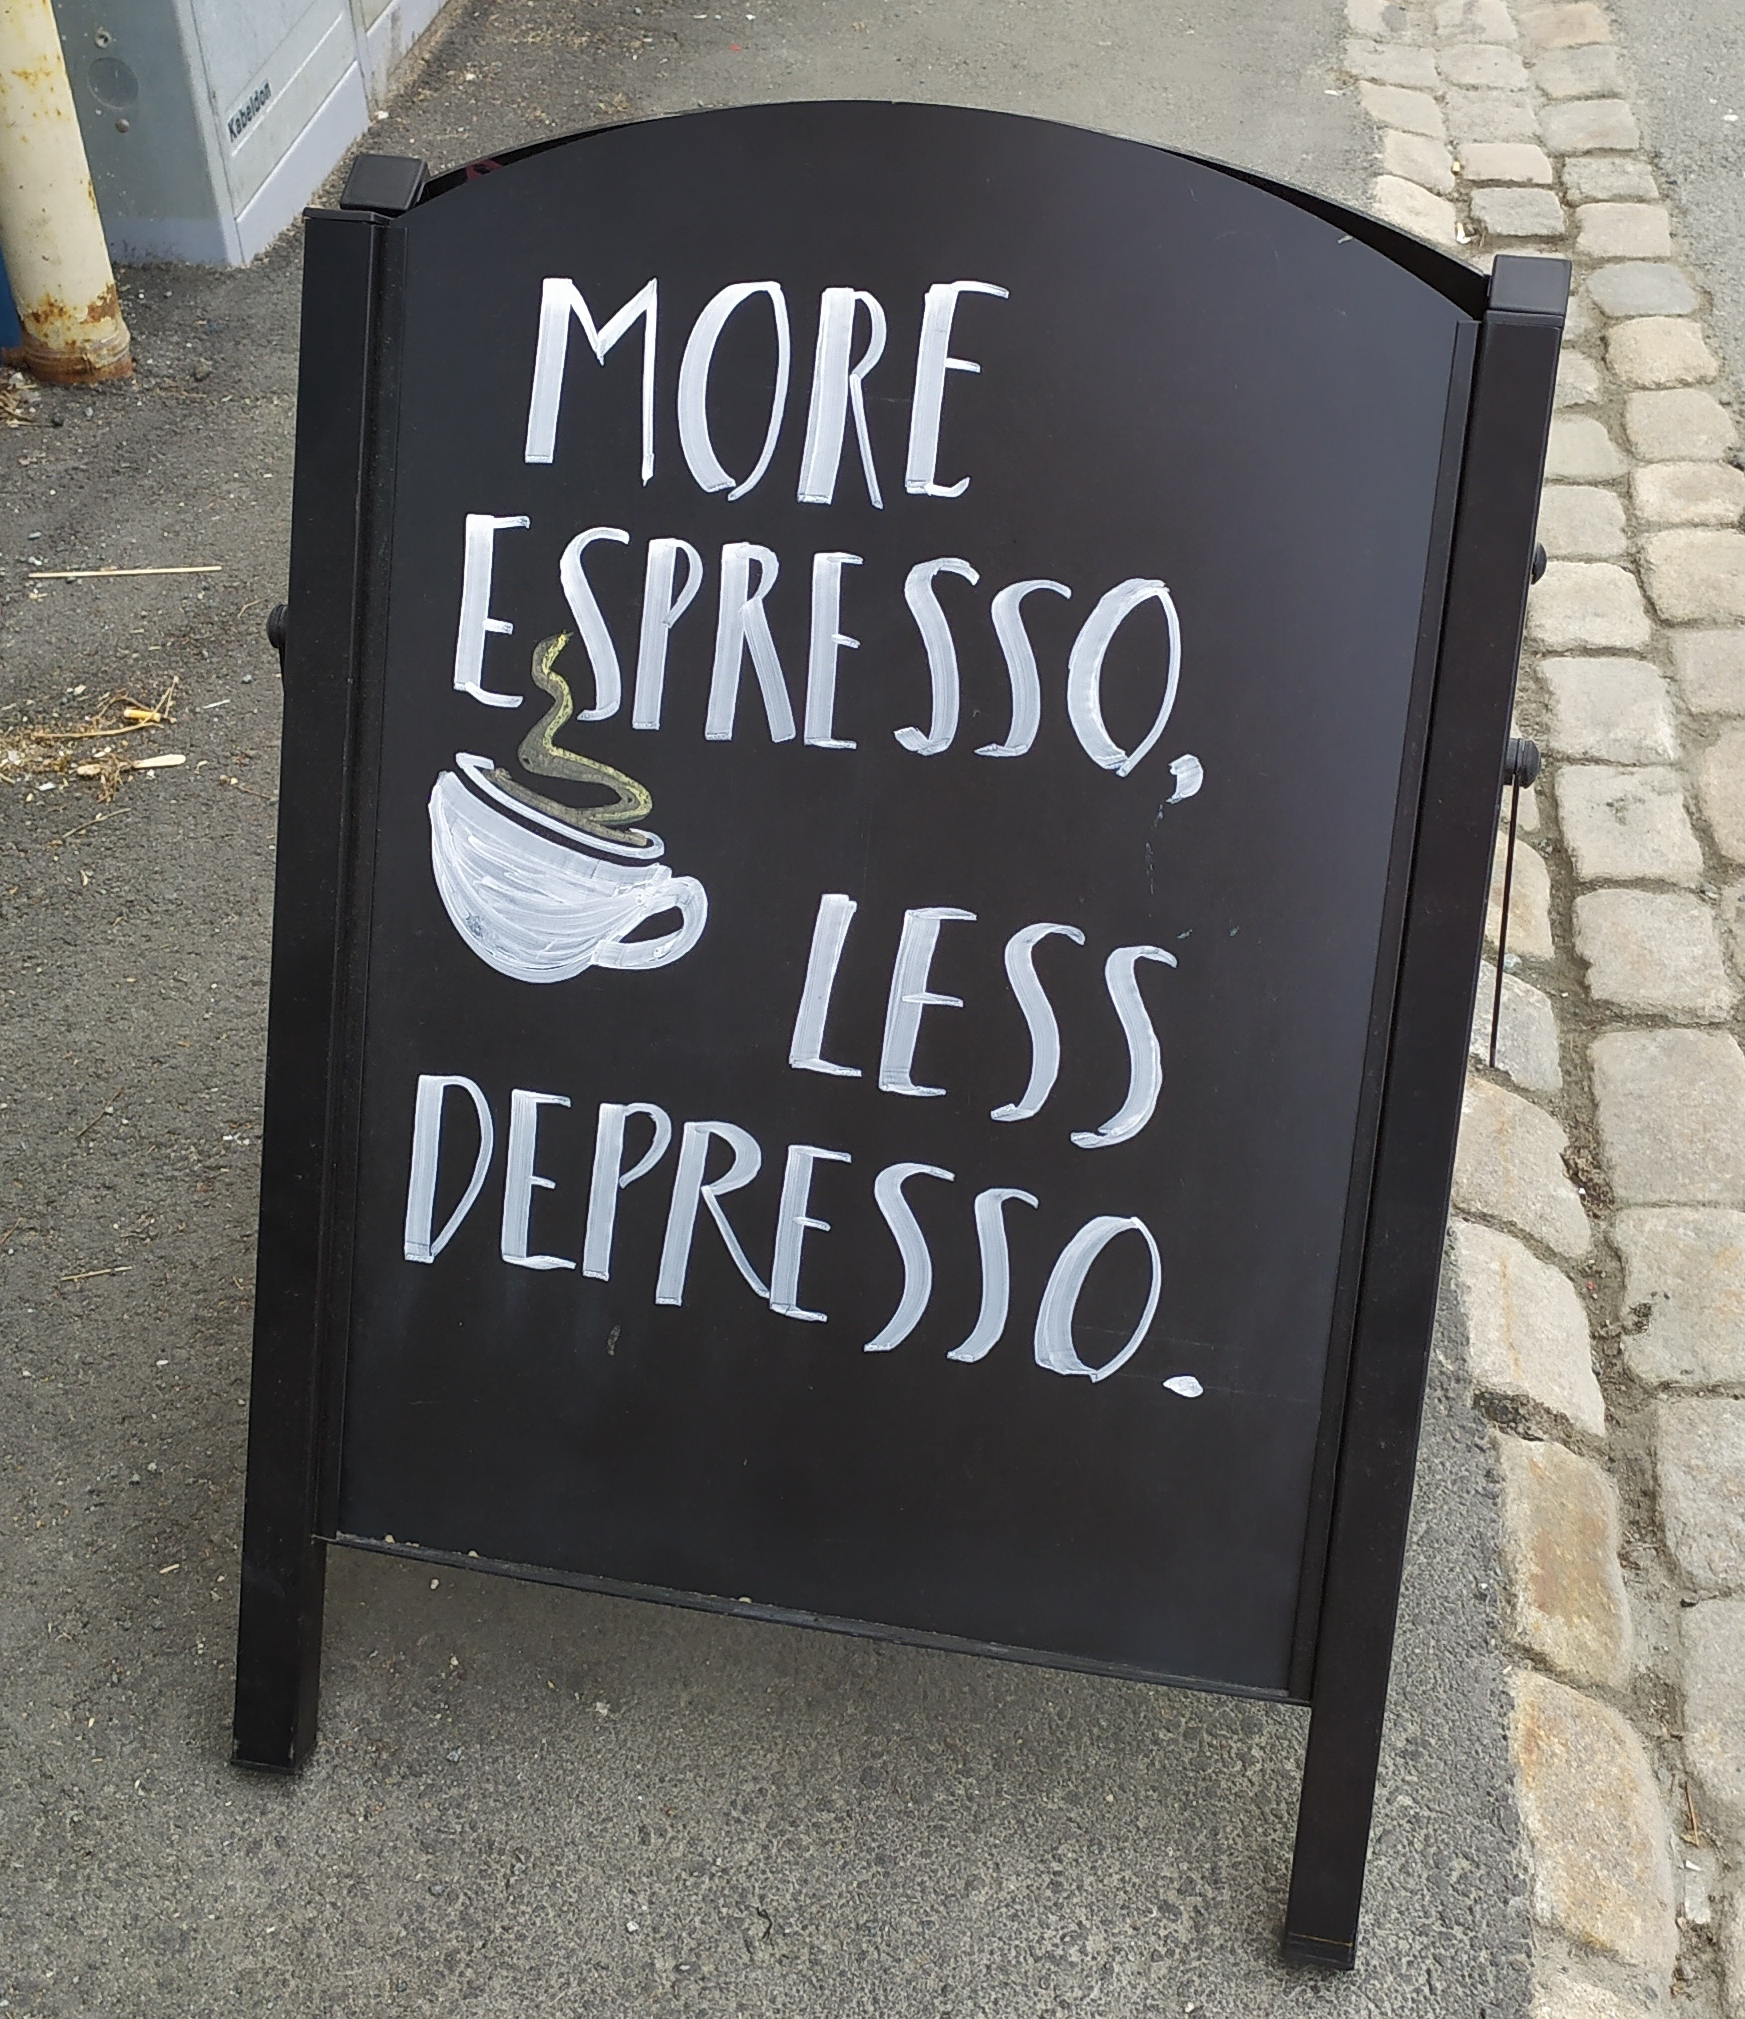
\includegraphics[width=0.4\linewidth]{img/depresso} \end{center}

\begin{right-align}
John Zobolas,
May 2021

\end{right-align}

\hypertarget{abstract}{%
\chapter*{Abstract}\label{abstract}}
\addcontentsline{toc}{chapter}{Abstract}

\vspace{-20pt}

Cancer is one the most prevalent human diseases.
The scientific community has devoted considerable efforts to understand the mechanisms behind this disease and search for treatments that promise a better quality of life for patients.
To accomplish this goal, Biology and Medicine have joined forces with Computer Sciences, using the power of Computational modeling, Mathematics, Machine Learning and Statistics.
This interdisciplinary effort to address the cancer problem, constitutes the basis upon which this thesis was formed.
We present several contributions to this effort, consisting of software, data analyses and mathematical investigations, which have enabled the more efficient curation of biological knowledge, the use of computer models to prioritize drug treatments for cancer and the derivation of molecular mechanistic insights from the simulation results.

In order to build a computational model of a biological system such as a cancer cell, we first need a way to describe the structure of such a system.
A common network-based approach provides an elegant representation of such a structure, where molecular entities such as proteins and genes are connected to each other via causal interactions, which in turn determine cellular behavior and the functional properties of the cell as an integrated system of individual components.
These interactions form the Prior Knowledge Network (PKN), which serves as the basic building block for most computational biological models. Nonetheless, several challenges exist, even at this early stage of the modeling process.

The first problem is that biological information by its very nature is largely complex, and therefore its formalization to a structured, computable form for use in modeling applications, demands extra attention.
The translation of scientific knowledge from publications into such a computable form is achieved with the use of specialized software tools and is the main responsibility of biocurators.
In order to help biocurators be more efficient in their annotation tasks, we proposed the Visual Syntax Method (VSM) as an alternative approach for general-purpose knowledge formalization.
In particular, we implemented a user interface component (VSM-box) that enables curators to annotate any type of information, no matter its complexity, and translate it into an intuitive, flexible sentence-like format.
This software was used to build a prototype curation interface (CausalBuilder) for the annotation of molecular causal interactions, which constitute the cornerstone of a model's PKN.

The second problem concerns the availability and ease of access of causal molecular interaction data for modeling or other scientific endeavors.
A standard format for the representation of such signaling information was developed (CausalTAB), and we supported the export of the causality statements from CausalBuilder's interface to this format.
But there exist several other molecular interaction databases that could update their data to fit the new CausalTAB standard.
PSICQUIC is a web-service platform that was initially built so that users can conveniently fetch in a standard way molecular interaction data from different sources.
We extended PSICQUIC to incorporate the new CausalTAB format, so that causality-enriched information generated by our curation prototype tool or from other data providers could be shared through a common channel.

A third major problem arose during the design process of the VSM-box and it's application, CausalBuilder.
Behind the scenes, the curator interface has to communicate with a large number of diverse biological data resources, each with its own online API service that provides access to the respective data.
In order to present to the user the available terms that pertain to a specific annotation of interest, a uniform way to query all these resources was needed.
This prompted us to build the Unified Biological Dictionaries (UBDs), a software suite that provides a unified gateway for life science data, helping users retrieve the right query terms.
In addition, curators sometimes come across new knowledge that is not yet available through the standard authoritative resources.
To address this related problem, we connected UBDs with PubDictionaries, an online resource of simple dictionaries, allowing curators to publicly create and share ad-hoc terms, and further use them as annotations in VSM-based applications.

After the signaling information has been curated and the causal interactions assembled to form the PKN, we then need to specify the mathematical equations of the cancer cell model.
This allows us to describe and analyze its dynamical behavior subject to external stimuli, such as drug perturbations.
The modeling approaches can in general range from qualitative to quantitative and in this work we focused on Boolean modeling, where signaling components are assigned either an active or inactive state.
An automated computational pipeline was developed to produce an ensemble of Boolean models from a PKN, calibrated to a specific cancer cell signaling phenotype.
These models are then analyzed to suggest possible synergistic drug combinations and the results are compared with experimental findings, where all possible combinations are tested in a high-throughput screen setup.
We demonstrated that our pipeline could prioritize specific drug combinations, reducing the number of drugs that need to be tested in experiments, before a viable treatment is found for a patient.
Moreover, several analyses indicated that our models can be used to derive mechanistic insights about the diseased model and generate novel biological hypotheses.
Lastly, we showed the significance of the PKN quality, where even small modifications to the cancer signaling network could severely affect our pipeline's drug prediction performance.

\newpage

To exploit the range of parameterizations present in the Boolean models produced by our pipeline, we devised several strategies to split and compare the different models in a dedicated R package (emba).
This supplementary effort allowed us to find potential biomarkers, which are nodes whose state is decisive for the global behavior of the models and can indicate parts of the PKN that are responsible for a drug combination to be synergistic.
Additionally, we noticed particular patterns in the way specific equations always correspond to specific signaling states in our models, so we more deeply investigated the influence of the choice of parameterization on the output behavior of these nodes.
This led us to propose a list of Boolean function metrics that can assist modelers in choosing more appropriate equations, meaning those that are consistent with the regulatory information present in the PKN and whose expected output better matches experimental observations.
Finally, results from a study of diverse Boolean functions indicated that these also exhibit diverse output behaviors, with some being highly biased towards specific Boolean outcomes while others depending more on the ratio between positive and negative regulators, as these are derived from the two distinct types of causal interactions present in the model's PKN.

\hypertarget{paper-list}{%
\chapter*{Paper list}\label{paper-list}}
\addcontentsline{toc}{chapter}{Paper list}

\hypertarget{primary}{%
\section*{Primary}\label{primary}}
\addcontentsline{toc}{section}{Primary}

Papers that I am first author:

\begin{itemize}
\item
  \textbf{Paper 1}: \emph{UniBioDicts: Unified access to Biological Dictionaries}\\
  \textbf{Zobolas, J.}, Touré, V., Kuiper, M., \& Vercruysse, S. {[}\protect\hyperlink{ref-UBDs}{1}{]}

  SV and VT identified the need for software to connect with the resources listed in MI2CAST used in the CausalBuilder tool. JZ implemented the software and wrote the manuscript. All co-authors revised and provided inputs to the manuscript.
\item
  \textbf{Paper 2}: \emph{Linking PubDictionaries with UniBioDicts to support Community Curation}\\
  \textbf{Zobolas, J.}, Kim, J.-D., Kuiper, M., \& Vercruysse, S. {[}\protect\hyperlink{ref-Zobolas2020-pubdict}{2}{]}

  MK and SV developed the original idea for this project. JZ wrote the application for a BioHackathon project and invited JDK to collaborate. JZ implemented the client side, JDK the server side. JZ wrote the manuscript. All co-authors revised and provided inputs to the manuscript.
\item
  \textbf{Paper 3}: \emph{emba: R package for analysis and visualization of biomarkers in Boolean model ensembles}\\
  \textbf{Zobolas, J.}, Kuiper, M., \& Flobak, Å. {[}\protect\hyperlink{ref-Zobolas2020}{3}{]}

  AF developed the idea of this project. JZ wrote the software and the manuscript. All co-authors revised and provided inputs to the manuscript.
\end{itemize}

\newpage

\begin{itemize}
\item
  \textbf{Paper 4}: \emph{Fine tuning a logical model of cancer cells to predict drug synergies: combining manual curation and automated parameterization}\footnote{(Manuscript) Shared first co-authorship, to be submitted to the Molecular Systems Biology Journal}\\
  Flobak, Å., \textbf{Zobolas J.}, Vazquez M., Steigedal T., Thommesen L., Grislingås A., Niederdorfer B., Folkesson E., Kuiper M.

  AF designed the project, developed initial software and executed experiments. JZ extended the software, ran all simulations, produced and analyzed results. AF and MK added biological interpretation and wrote the manuscript. JZ provided various inputs and text to the manuscript. TS, LT and AG helped AF with experiments. MV developed prototype software. BN and EF did curation work and performed experiments.
\item
  \textbf{Paper 5}: \emph{Boolean function metrics can assist modelers to check and choose logical rules}\footnote{(Preprint) To be submitted to the Journal of Theoretical Biology}\\
  \textbf{Zobolas, J.}, Monteiro, P. T., Kuiper, M., \& Flobak, Å. {[}\protect\hyperlink{ref-Zobolas2021-bias}{4}{]}

  JZ designed this project and wrote the manuscript. PTM and AF provided feedback and ideas to better shape the content of the manuscript. All co-authors revised and provided inputs to the manuscript.
\end{itemize}

\hypertarget{additional}{%
\section*{Additional}\label{additional}}
\addcontentsline{toc}{section}{Additional}

In the following papers I have contributed to the underlying software and manuscript text:

\begin{enumerate}
\def\labelenumi{\arabic{enumi}.}
\tightlist
\item
  \emph{VSM-box: General-purpose Interface for Biocuration and Knowledge Representation}\\
  Vercruysse, S., \textbf{Zobolas, J.}, Touré, V., Andersen, M. K., \& Kuiper, M. {[}\protect\hyperlink{ref-vsm-box}{5}{]}
\item
  \emph{CausalBuilder: Bringing the MI2CAST Causal Interaction Annotation Standard to the Curator}\\
  Touré, V., \textbf{Zobolas, J.}, Kuiper, M., \& Vercruysse, S. {[}\protect\hyperlink{ref-Toure2021}{6}{]}
\item
  \emph{CausalTAB: the PSI-MITAB 2.8 updated format for signalling data representation and dissemination}\\
  Perfetto, L., Acencio, M. L., Bradley, G., Cesareni, G., Del Toro, N., Fazekas, D., Hermjakob, H., Korcsmaros, T., Kuiper, M., Lægreid, A., Lo Surdo, P., Lovering, R. C., Orchard, S., Porras, P., Thomas, P. D., Touré, V., \textbf{Zobolas, J.}, \& Licata, L. {[}\protect\hyperlink{ref-Perfetto2019}{7}{]}
\end{enumerate}

\hypertarget{abbreviations}{%
\chapter*{Abbreviations}\label{abbreviations}}
\addcontentsline{toc}{chapter}{Abbreviations}

\begin{longtable}{ll}
\toprule
abmlog & All possible Boolean Models Link Operator Generator\\
AGS & Gastric Adenocarcinoma (cell line)\\
API & Application Programming Interface\\
AUC & Area Under the Curve\\
BioPax & Biological Pathway Exchange\\
\addlinespace
CASCADE & CAncer Signaling CAusality DatabasE\\
CNA & Copy Number Alterations\\
COVID-19 & COrona VIrus Disease 2019\\
drabme & Drug Response Analysis to Boolean Model Ensembles\\
emba & Ensemble (Boolean) Model Biomarker Analysis\\
\addlinespace
gitsbe & Generic Interactions To Specific Boolean Equations\\
GO & Gene Ontology\\
GREEKC & Gene Regulation Ensemble Effort for the Knowledge Commons\\
HUPO-PSI & HUman Proteome Organization - Proteomics Standards Initiative\\
IMEx & The International Molecular Exchange Consortium\\
\addlinespace
MI2CAST & Minimum Information about a Molecular Interaction CAusal STatement\\
MIQL & Molecular Interactions Query Language\\
MITAB & Molecular Interaction TABular format\\
ODE & Ordinary Differential Equation\\
PDE & Partial Differential Equation\\
\addlinespace
PKN & Prior Knowledge Network\\
PPI & Protein-Protein Interaction\\
PRC & Precision Recall Curve\\
PSICQUIC & Proteomics Standard Initiative Common QUery InterfaCe\\
ROC & Receiver Operating Characteristic\\
\addlinespace
SBGN & Systems Biology Graphical Notation\\
TF-TG & Transcription Factor - Target Gene\\
UBDs (UniBioDicts) & Unified Biological Dictionaries\\
UMAP & Uniform Manifold Approximation and Projection (for dimension reduction)\\
VSM & Visual Syntax Method\\
\addlinespace
XML & Extensible Markup Language\\
\bottomrule
\end{longtable}

\mainmatter

\hypertarget{summary}{%
\chapter*{Summary}\label{summary}}
\addcontentsline{toc}{chapter}{Summary}

\hypertarget{one-for-all}{%
\section*{One for all}\label{one-for-all}}
\addcontentsline{toc}{section}{One for all}

Scientific and technological progress has been the foundation for some of the most astounding achievements of humankind.
In the last century in particular, discoveries were made that contributed to the sustainable development of the economy and society, affecting our lives in an unprecedented manner and making possible what was considered impossible.
The invention of the digital computer and the Internet for example, revolutionized the access, dissemination and analysis of information {[}\protect\hyperlink{ref-Abbate2000}{8},\protect\hyperlink{ref-Naughton2016}{9}{]}.
We have been to the Moon, a breakthrough that has opened up the possibilities of space exploration and interstellar travel.
The industrial revolution of the latest century has enabled us to design machines for every conceivable need.
Human well-being has become significantly better: compare a middle class household and the appliances within, with one from 60 years ago.
With a higher standard of living and the ongoing efforts to alleviate hunger, poverty and inequality on a global scale, people have started caring more about the planet, paving the way for sustainable economic and environmental growth {[}\protect\hyperlink{ref-Polasky2019}{10}{]}.
Due to advancements in Biology and Medicine, the application of public health interventions such as vaccinations and hygiene measures has become common practice, causing a rapid increase in the global life expectancy during the last century {[}\protect\hyperlink{ref-Roser2013}{11}{]}.
The genome-editing technology CRISPR {[}\protect\hyperlink{ref-Jinek2012}{12}{]} has enabled the discovery of new therapeutic solutions for a variety of genetic diseases and has been beneficially used in several agriculture and plant biotechnology applications {[}\protect\hyperlink{ref-Zhu2020}{13}{]}.
The list of achievements is truly endless and all the data points to the fact that the world is getting better {[}\protect\hyperlink{ref-Bailey2020}{14}{]}.

There are three factors that have made technological progress possible.
Firstly, every human innovation is based on basic scientific research, without which the development of new technologies would have been impossible.
Secondly, society is developing new contracts with science {[}\protect\hyperlink{ref-Gibbons1999}{15}{]}, where researchers can only be trusted to continue their work (and get funding for it), if they tackle real-world problems and produce knowledge characterized by a fully transparent and participative spirit.
Practically, this means that better communication skills are a necessity for today's scientists and that their research should have translational potential to deliver on society's expectations.
But solving these real-world problems is incredibly hard, and so, they cannot be addressed by applying knowledge from specific fields only, e.g.~either from the Computer or the Biological Sciences alone.
This brings us to the third factor: in order for science to deliver on its promises to society, collaboration across fields of science is the only way forward.

Medicine, from research to develop new therapies up to delivering the actual product or services to the patients, constitutes the perfect example that encompasses all three reasons that have enabled progress to transpire in its domain.
It first starts with a real-life problem: people get sick.
The existence of diseases is a societal problem and a hard one at that, since people usually lack the necessary knowledge or the means to deal with it on their own.
They have in fact exchanged some of their freedom to have a place in society, and ensure that they receive proper treatment when needed (along with other forms of security, access to free education, etc.).
To manage such a complex problem, society provides healthcare services, which have significantly increased across the world in recent years {[}\protect\hyperlink{ref-HAQ2015}{16}{]}.
For most people, the single most applied healthcare interaction is the use of drugs, prescribed by medical doctors.
Drugs are the translational product of the pharmaceutical industry, which is the result of basic interdisciplinary research.
Medical doctors alone wouldn't be able to find the cause and understand the mechanisms behind many of the diseases that exist today.
This knowledge has been the culmination of years of scientific knowledge, built atop collaboration across fields, from Medicine and Biology to Computer Science and Engineering.

So, only by using every possible method and knowledge at our disposal and by working together, we can achieve the solution to complex problems such as human diseases.
When these conditions are met, societal challenges can be addressed and science stands as one unified body for the good and progress of all mankind.
The field of Systems Medicine has been the direct embodiment of this notion, promising improved prevention, prognosis, diagnosis and treatment of patients via an integrative, interdisciplinary approach {[}\protect\hyperlink{ref-Apweiler2018}{17}{]}.

\newpage

\hypertarget{dots-and-lines}{%
\section*{Dots and lines}\label{dots-and-lines}}
\addcontentsline{toc}{section}{Dots and lines}

One of the simplest ways to conceptualize complex systems, either man-made or existing freely in nature, is using the notion of a \emph{network} or \emph{graph}.
The idea is that any system is composed of individual entities or components of interest (nodes) and these components interact with each other in various, usually non-obvious ways (links).
These two properties, namely having some objects to study, and relationships between these objects, form the basis for the conceptualization of a network (Figure \ref{fig:fig1}).
From a cognitive point of view, the conceptualization of a network manifests as a visual representation in our brain, consisting of a bunch of dots (nodes) connected with numerous lines (links) {[}\protect\hyperlink{ref-Trudeau1976}{18}{]}.
Such a projection is usually close to what people instinctively draw on paper when they attempt to describe their knowledge about a system and its inner workings (thereby ``connecting the dots'').
Simple schematics that are abstractly similar to dots and lines, along with further contextual information (e.g.~node labels, coloring, directed links, etc.), seem to be able to capture and render information derived from our thought processes, in a unique and comprehensible way.



\begin{figure}
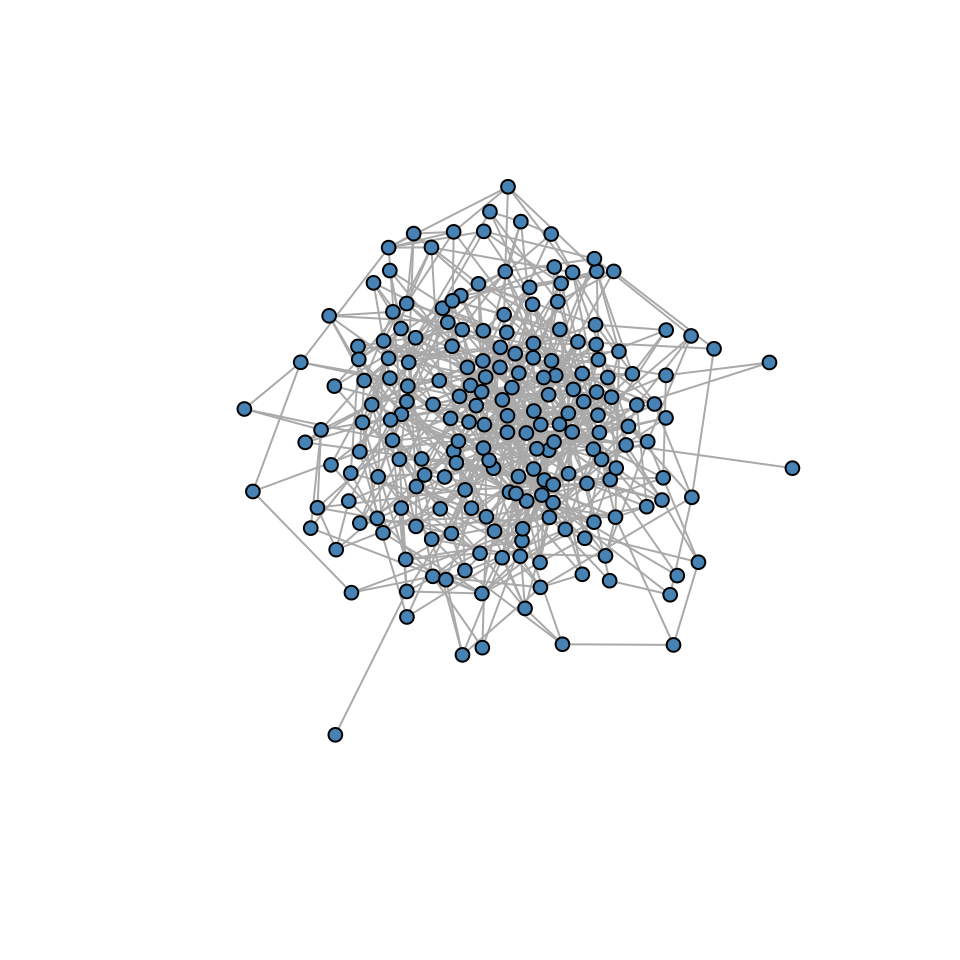
\includegraphics[width=0.5\linewidth]{phd-thesis_files/figure-latex/fig1-1} 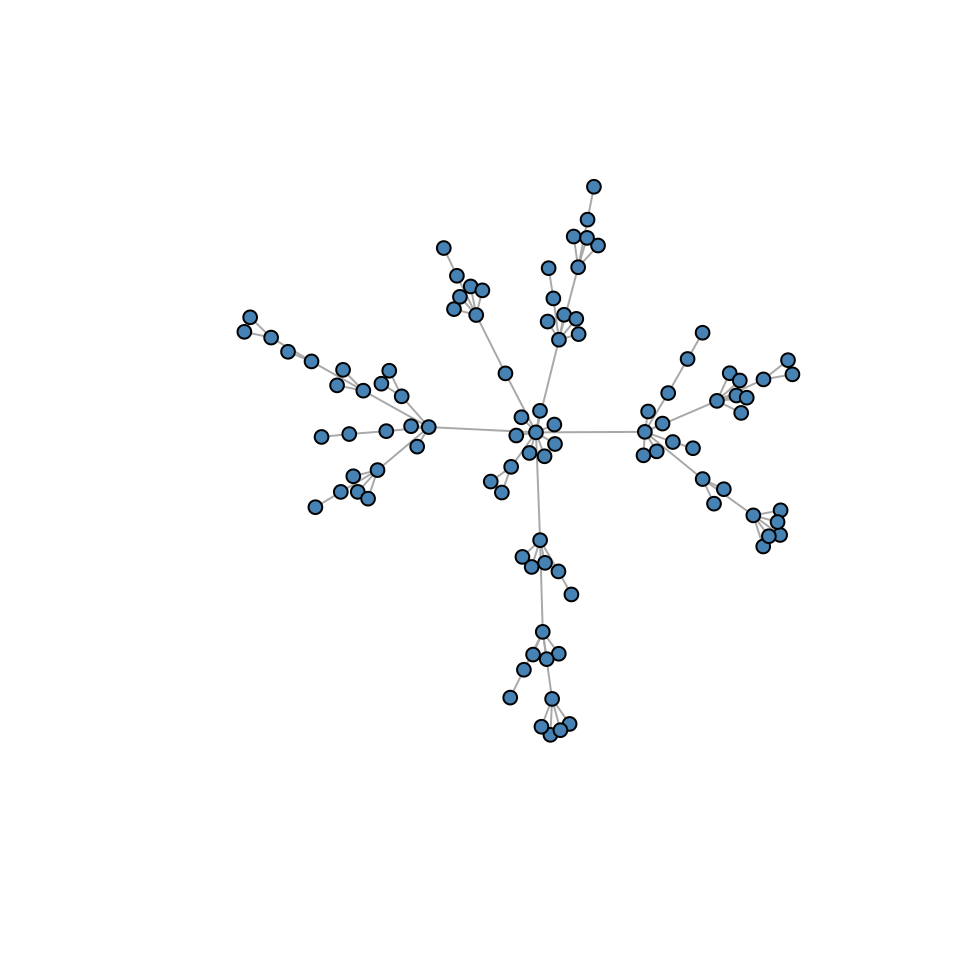
\includegraphics[width=0.5\linewidth]{phd-thesis_files/figure-latex/fig1-2} \caption{Two examples of networks, composed of dots and lines. The left network is a random graph based on the Erdős--Rényi model {[}\protect\hyperlink{ref-Erdos1960}{19}{]} and the one on the right is created using the preferential attachment principle that characterizes scale-free networks with hub nodes, such as the World Wide Web {[}\protect\hyperlink{ref-Barabasi1999}{20}{]}.}\label{fig:fig1}
\end{figure}

Since studying complex systems falls intro the domain of science's responsibilities, and graphs seem to be an intuitive way of representing such systems, the emergence of a new field called network science was inevitable {[}\protect\hyperlink{ref-Barabasi2013}{21}{]}.
Its purpose is to establish a unified set of tools and methods to study the properties of any type of network that emerges across disparate fields.
A variety of software tools for network visualization and analysis have been released throughout the years, ranging from generic-purpose {[}\protect\hyperlink{ref-Csardi2006}{22}--\protect\hyperlink{ref-Shannon2003}{25}{]}, to tools more suitable for studying biological {[}\protect\hyperlink{ref-Dahlquist2002}{26}--\protect\hyperlink{ref-Sidiropoulos2017}{29}{]} or social networks {[}\protect\hyperlink{ref-Smith2009}{30},\protect\hyperlink{ref-Kalamaras2014}{31}{]}.
The use of such tools enables the discovery of fundamental laws that characterize the function of systems represented by networks.
In addition, it allows us to study in detail the networks' systemic structure and derive key principles that drive their evolution and emergent behavior.
Anthropological research for example uses network theory to study people and their relationships, and explain emergent complex phenomena such as human behavior.
Neuroscience uses network analysis methods to detect anomalies in diseased human brains {[}\protect\hyperlink{ref-Chatterjee2021}{32}{]}.
The impact of online social networks is studied to understand and predict future personal and profit-oriented communication (online marketing) {[}\protect\hyperlink{ref-Mislove2007}{33}{]}.
Epidemiologists use graph-based methods to model the spread of diseases like COVID-19, predict the future course of outbreaks and evaluate strategies to control epidemics {[}\protect\hyperlink{ref-Maheshwari2020}{34}{]}.
Molecular biologists study intra- and intercellular signaling networks to understand the mechanisms behind biological processes and investigate the causes of network dysregulation, often leading to the emergence of particular disease phenotypes.
Such network-based approaches have significant clinical applications since they have the potential to assist in the discovery of new disease genes and modules, and the identification of drug targets and biomarkers for complex diseases {[}\protect\hyperlink{ref-Barabasi2011}{35}{]}.

The work presented in this thesis is heavily based on this network medicine paradigm, with causal molecular interaction networks as the main object of study.
Our primary focus is on protein-protein interaction (PPI) networks, with proteins as nodes and their physical contacts and interactions as links, and gene regulatory networks, represented for example by directed regulatory relationships between transcription factors and genes (TF-TG networks).
These types of networks demonstrate a system of signal transduction pathways connected by crosstalk and embedded in feedback loops, forming what is known as the \emph{Prior Knowledge Network} (PKN).
The causality property of the PKN stems from the fact that the network links are directed (i.e.~protein X affects protein Y) and signed (Y is inhibited or activated as a result).
It's exactly this causality information that allows the investigation of behaviors from a systems perspective.
Such networks form the basis for the study and computational modeling of cancer, which is another subject of investigation in this thesis.
In the subsequent chapters, we will discuss how we addressed problems related to the formalization, access and public sharing of the knowledge encoded in the PKN.

\newpage

\hypertarget{knowledge-from-a-stack-of-papers}{%
\section*{Knowledge from a stack of papers}\label{knowledge-from-a-stack-of-papers}}
\addcontentsline{toc}{section}{Knowledge from a stack of papers}

Where does the information that is used to build knowledge networks originate from?
One of the most widely adopted ways to record and share knowledge, has been the publication of scientific findings in specialized journals.
This has resulted in a major challenge that researchers in the life sciences face, which is to stay updated with the huge amount of information that is published on a daily basis (Figure \ref{fig:fig2}).
It becomes impossible for the average scientist to find, read, extract and use that information in an efficient manner without the use of databases.
Even when using databases, one is often confronted with both chronically incomplete knowledge, and also a lack of sufficient contextual information to assess when exactly the knowledge is valid.



\begin{figure}

{\centering 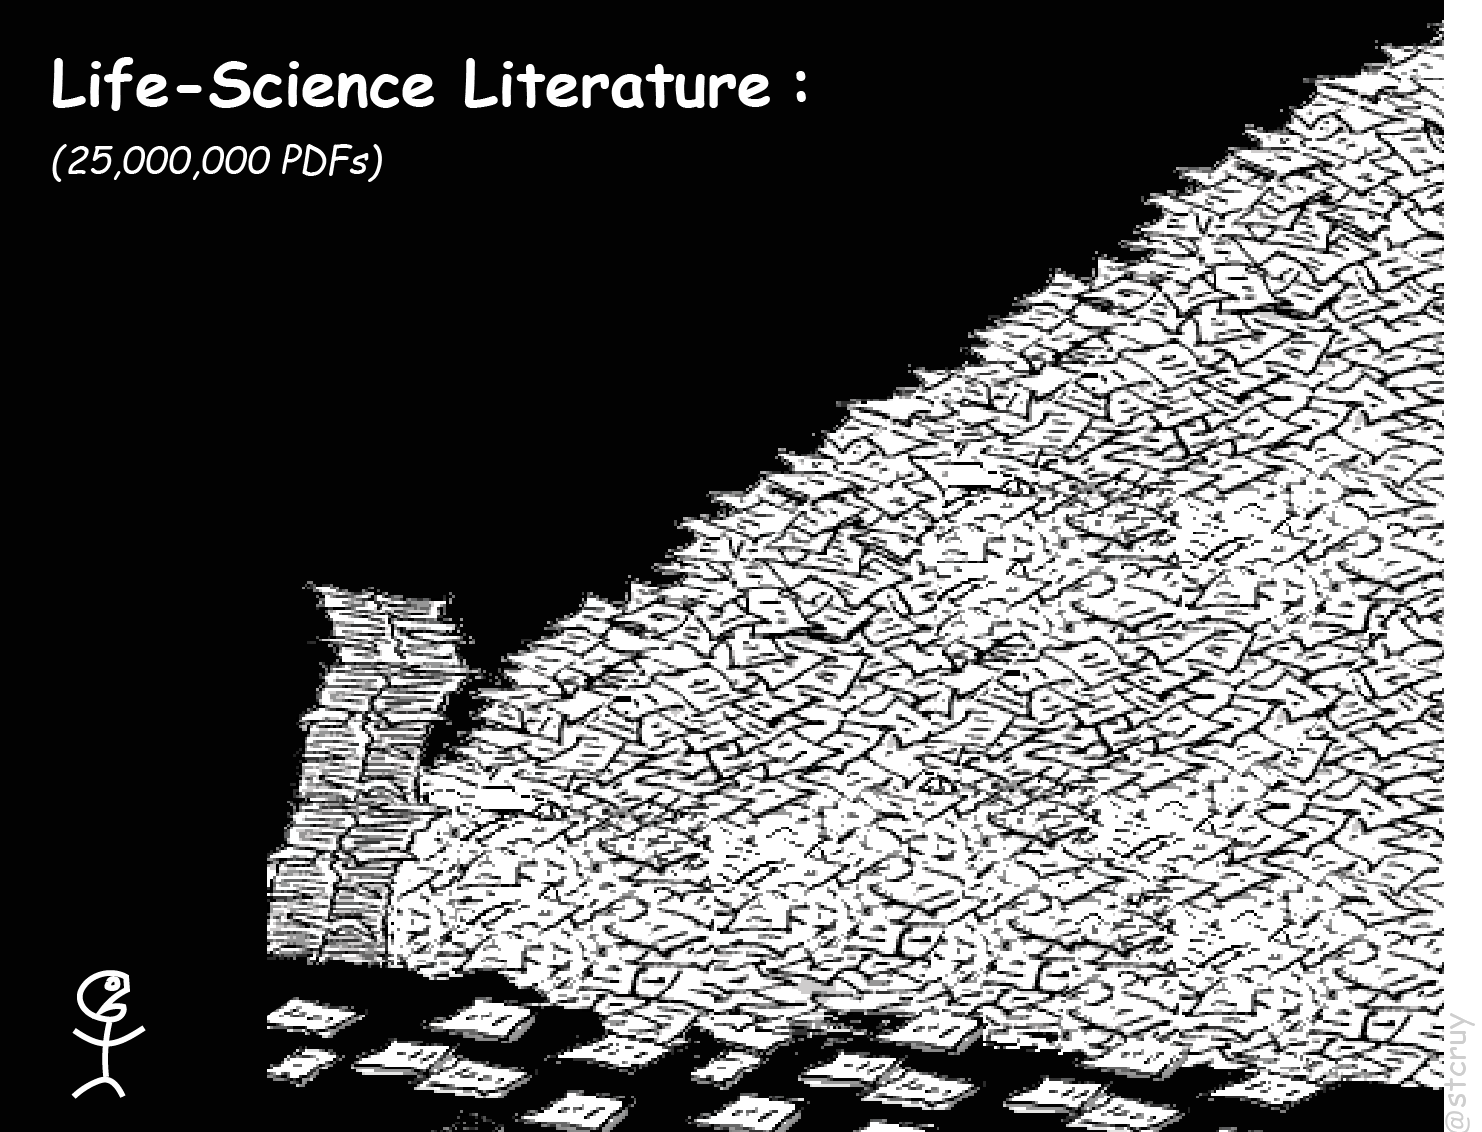
\includegraphics[width=0.75\linewidth]{img/papers} 

}

\caption{Human vs Life-Science Literature. How can humans stay up-to-date with increasing knowledge stored in PDF files? {[}\protect\hyperlink{ref-Vercruysse2019a}{36}{]}}\label{fig:fig2}
\end{figure}

A severe problem lies already at the data entry stage.
Biocurators are people whose main task is to read the scientific literature and translate knowledge into a precise, computable form, ready to be inserted into databases {[}\protect\hyperlink{ref-Howe2008}{37},\protect\hyperlink{ref-Ammari2018}{38}{]}.
The huge body of literature existing today is full of inconsistencies and inaccuracies, so expert interpretation and annotation are essential.
But current databases are limited in what they can contain, because there exists no easy way to properly transfer all kinds of complex knowledge or ideas into them, in the first place.
Moreover, the annotation tools that biocurators use are not intuitive nor flexible enough to be used by large crowds of people, to convert vast amounts of relevant knowledge from the scientific literature into the respective databases.
The insufficient funding to curate scientific results into databases, and the cost of creating a new knowledge base for every new project, are some extra confounding factors.
Because of this, researchers all over the world have to spend considerable time performing ad-hoc manual curation of publications that are relevant for their project, often with improvised approaches (Word, Excel).
At best they also spend time developing a specialized curation platform or computational methods to extract knowledge, which can only capture a fraction of the ``actual reported truth'' {[}\protect\hyperlink{ref-Jenssen2001}{39}{]}.
Nonetheless, all these efforts form a significant part of the scientific enterprise, assisting in the creation of digital knowledge repositories, which are subsequently used to build PKNs for the computational modeling of biological processes.

\vspace{15pt}

A list of tools have been created to assist biocurators in their annotation tasks.
Notably, the IntAct editor is an open-source desktop application software that enables IntAct curators and members of the IMEx consortium to annotate molecular interactions {[}\protect\hyperlink{ref-intact-editor}{40}{]}.
Because of the lack of installation instructions and documentation, coupled with a complex interface, specialized training from senior IntAct curators is required to learn how to use this software.
Nonetheless, it is one of the most used and effective tools for the job, since it has been around for a lot of years and during that time, there has always been a spirit of close collaboration between developers and curators to implement features, solve bugs and in general improve the annotation capabilities of the software.
Canto is another tool that was built to support community curation in the PomBase fission yeast database {[}\protect\hyperlink{ref-Rutherford2014}{41}{]}.
It has now expanded its original purpose to support curation of other model organism databases and different molecular data types (e.g.~annotation of a larger set of GO terms).
Canto's respective website provides extensive documentation and step-by-step user guidance throughout the annotation procedure {[}\protect\hyperlink{ref-canto-doc}{42}{]}.
A user management mechanism is incorporated in the software so as to allow proper monitoring of curation tasks and efficient communication between curators for work prioritization.
In addition, two relatively new tools have been developed for the curation and visualization of molecular interaction maps: NaviCell {[}\protect\hyperlink{ref-Kuperstein2013}{43}{]} and MINERVA {[}\protect\hyperlink{ref-Gawron2016}{44}{]}.
These tools facilitate knowledge exploration in addition to knowledge annotation, allowing for an interactive user experience (e.g.~feedback via comments), enabling content sharing, supporting well known data standards (e.g.~SBGN {[}\protect\hyperlink{ref-Novere2009}{45}{]}) and thus allowing for data interoperability and re-use.
All the aforementioned annotation tools are limited by the fact that they aren't generic enough to curate any type of information, with most of them representing specialized solutions pertaining to specific annotation purposes.
Most tools require extra technical configurations and software to include additional levels of contextualized details required for current and future curation efforts.

\newpage

To obtain support from computational pipelines that will help us process the vast amounts of knowledge and advance our understanding of processes in nature, we must be able to efficiently annotate and store information that is highly detailed and contextualized.
Hereby, the knowledge's inherent complexity should be kept manageable and understandable by humans and machines alike.
In order to accommodate for a much more powerful, flexible, and reusable annotation process, an intuitive curation and knowledge formalization method was developed, called VSM (Visual Syntax Method) {[}\protect\hyperlink{ref-vsm-paper}{46}{]}.
VSM enables scientists to capture any type of knowledge with any type of contextual information, in a way that is understandable by both humans and computers.

Part of the work in this thesis has been to assist in the implementation of a software module that implements VSM as a general-purpose, web-based user interface, named VSM-box {[}\protect\hyperlink{ref-vsm-box}{5}{]}.
This software component was used to build CausalBuilder, a prototype curation interface for the annotation of causal molecular interactions {[}\protect\hyperlink{ref-Toure2021}{6}{]}.
CausalBuilder uses VSM to generate concrete, customizable templates that represent causal statements.
It supports the export of the annotated statements in standard signaling formats, such as CausalTAB {[}\protect\hyperlink{ref-Perfetto2019}{7}{]}, which can be stored in relevant databases or used to build computational models of biological processes.
To support the large variety of contextual information related to causal molecular interactions between biological entities, allowing for a finer disambiguation between seemingly similar or conflicting causality statements (e.g.~a transcription factor simultaneously up and down regulating a target gene in different cellular contexts), CausalBuilder was designed to comply with a list of guidelines (MI2CAST) that were developed exactly for this purpose {[}\protect\hyperlink{ref-Toure2020}{47}{]}.
All in all, CausalBuilder provides biologists and curators with a simple user interface for the annotation of causal regulatory knowledge, translating highly contextual information about molecular interactions from scientific publications to a computable form.

\newpage

\hypertarget{biological-dictionaries-aid-in-the-curation-of-complex-knowledge}{%
\section*{Biological Dictionaries aid in the curation of complex knowledge}\label{biological-dictionaries-aid-in-the-curation-of-complex-knowledge}}
\addcontentsline{toc}{section}{Biological Dictionaries aid in the curation of complex knowledge}

\hypertarget{sharing-causal-interactions-with-psicquic}{%
\section*{Sharing causal interactions with PSICQUIC}\label{sharing-causal-interactions-with-psicquic}}
\addcontentsline{toc}{section}{Sharing causal interactions with PSICQUIC}

\hypertarget{biological-modeling-a-prelude}{%
\section*{Biological modeling: a Prelude}\label{biological-modeling-a-prelude}}
\addcontentsline{toc}{section}{Biological modeling: a Prelude}

\hypertarget{clean-code}{%
\section*{Clean Code}\label{clean-code}}
\addcontentsline{toc}{section}{Clean Code}

\hypertarget{appendix-appendix}{%
\appendix}


\hypertarget{links-to-software-documentation-and-data-analyses}{%
\chapter*{Links to software, documentation and data analyses}\label{links-to-software-documentation-and-data-analyses}}
\addcontentsline{toc}{chapter}{Links to software, documentation and data analyses}

\vspace{-10pt}

\hypertarget{github-org-links}{%
\section*{GitHub organizations}\label{github-org-links}}
\addcontentsline{toc}{section}{GitHub organizations}

\begin{itemize}
\tightlist
\item
  UniBioDicts: \url{https://github.com/UniBioDicts/}
\item
  VSM: \url{https://github.com/vsm}
\item
  DrugLogics: \url{https://github.com/druglogics}
\item
  PSICQUIC: \url{https://github.com/PSICQUIC}
\end{itemize}

\hypertarget{doc-links}{%
\section*{Documentation}\label{doc-links}}
\addcontentsline{toc}{section}{Documentation}

\begin{itemize}
\tightlist
\item
  DrugLogics software: \url{https://druglogics.github.io/druglogics-doc/}
\item
  VSM technology and related projects: \url{https://vsm.github.io/}
\item
  PSICQUIC: \url{https://psicquic.github.io/}
\end{itemize}

\hypertarget{druglogics-soft-links}{%
\section*{DrugLogics software modules}\label{druglogics-soft-links}}
\addcontentsline{toc}{section}{DrugLogics software modules}

\begin{itemize}
\tightlist
\item
  \href{https://github.com/druglogics/gitsbe}{\texttt{gitsbe}}: A Java module that defines Boolean models compliant with observed behavior (e.g.~steady state or perturbation data) using an automated, model parameterization genetic algorithm
\item
  \href{https://github.com/druglogics/drabme}{\texttt{drabme}}: A Java module that performs a drug perturbation response analysis to the Boolean model ensembles generated by gitsbe
\item
  \href{https://github.com/druglogics/druglogics-synergy}{\texttt{druglogics-synergy}}: A Java module to execute serially gitsbe and then drabme
\item
  \href{https://github.com/druglogics/abmlog}{\texttt{abmlog}}: A Java-based generator of all possible logical models with AND/OR-NOT link operators in their respective Boolean equations
\item
  \href{https://github.com/druglogics/druglogics-roc}{\texttt{druglogics-roc}}: \texttt{R} Shiny web app to visualize the ROC and PR prediction performance of drabme's ensemble-wise predictions
\item
  \href{https://github.com/bblodfon/emba/}{\texttt{emba}}: \texttt{R} package for analysis and visualization of biomarkers in Boolean model ensembles
\end{itemize}

\hypertarget{r-community-packages}{%
\section*{R community packages}\label{r-community-packages}}
\addcontentsline{toc}{section}{R community packages}

\begin{itemize}
\tightlist
\item
  \href{https://github.com/bblodfon/usefun}{\texttt{usefun}}: various useful \texttt{R} functions
\item
  \href{https://github.com/bblodfon/rtemps}{\texttt{rtemps}}: templates for reproducible data analyses with \texttt{R} {[}\protect\hyperlink{ref-rtemps}{48}{]}
\end{itemize}

\hypertarget{misc-links}{%
\section*{Miscellaneous data analyses and repositories}\label{misc-links}}
\addcontentsline{toc}{section}{Miscellaneous data analyses and repositories}

All the following repositories have been authored exclusively by myself.
Each repository has a \texttt{README.md} file with a brief description of the analysis and a link to online documentation and results (in the form of \texttt{R} Markdown documents or \texttt{R} GitBooks).

\begin{itemize}
\tightlist
\item
  \href{https://github.com/druglogics/cascade}{\texttt{CASCADE}}: repository of the CAncer Signaling CAusality DatabasE developed by the DrugLogics group and its subsequent versions
\item
  \href{https://github.com/druglogics/ags-paper}{\texttt{ags-paper}}: simulation results and data analyses related to the AGS paper manuscript
\item
  \href{https://github.com/druglogics/sintef-obs-synergies}{\texttt{sintef-obs-synergies}}: synergy assessment of the Flobak et al.~(2019) {[}\protect\hyperlink{ref-Flobak2019}{49}{]} drug combination dataset using rbbt {[}\protect\hyperlink{ref-Vazquez2010}{50}{]} and the CImbinator tool {[}\protect\hyperlink{ref-Flobak2017}{51}{]}
\item
  \href{https://github.com/druglogics/brf-bias}{\texttt{brf-bias}}: data analyses related to truth density bias in standardized Boolean regulatory functions (results are part of the Boolean function metrics paper)
\item
  \href{https://github.com/druglogics/gitsbe-model-analysis}{\texttt{gitsbe-model-analysis}}: several analyses using Boolean model ensemble datasets generated via gitsbe and the emba \texttt{R} package to analyze them
\item
  \href{https://github.com/druglogics/bool-param-maps}{\texttt{bool-param-maps}}: visualization of model parameterization and node importance using UMAP and random forests on the CASCADE 1.0 Boolean model dataset generated by \texttt{abmlog}
\end{itemize}

\hypertarget{references}{%
\chapter*{References}\label{references}}
\addcontentsline{toc}{chapter}{References}

\hypertarget{refs}{}
\begin{CSLReferences}{1}{0}
\leavevmode\hypertarget{ref-UBDs}{}%
1. Zobolas, J., Touré, V., Kuiper, M., \& Vercruysse, S. (2020). {UniBioDicts: Unified access to Biological Dictionaries}. \emph{Bioinformatics}, \emph{37}(1), 143--144. \url{https://doi.org/10.1093/bioinformatics/btaa1065}

\leavevmode\hypertarget{ref-Zobolas2020-pubdict}{}%
2. Zobolas, J., Kim, J.-D., Kuiper, M., \& Vercruysse, S. (2020). \emph{{Linking PubDictionaries with UniBioDicts to support Community Curation}}. BioHackrXiv. \url{https://doi.org/10.37044/osf.io/gzfa8}

\leavevmode\hypertarget{ref-Zobolas2020}{}%
3. Zobolas, J., Kuiper, M., \& Flobak, Å. (2020). {emba: R package for analysis and visualization of biomarkers in boolean model ensembles}. \emph{Journal of Open Source Software}, \emph{5}(53), 2583. \url{https://doi.org/10.21105/joss.02583}

\leavevmode\hypertarget{ref-Zobolas2021-bias}{}%
4. Zobolas, J., Monteiro, P. T., Kuiper, M., \& Flobak, Å. (2021). \emph{{Boolean function metrics can assist modelers to check and choose logical rules}}. \url{http://arxiv.org/abs/2104.01279}

\leavevmode\hypertarget{ref-vsm-box}{}%
5. Vercruysse, S., Zobolas, J., Touré, V., Andersen, M. K., \& Kuiper, M. (2020). {VSM-box: general-purpose interface for biocuration and knowledge representation}. \emph{Preprints}. \url{https://doi.org/10.20944/preprints202007.0557.v1}

\leavevmode\hypertarget{ref-Toure2021}{}%
6. Touré, V., Zobolas, J., Kuiper, M., \& Vercruysse, S. (2021). {CausalBuilder: bringing the MI2CAST causal interaction annotation standard to the curator}. \emph{Database}. \url{https://doi.org/10.1093/database/baaa107}

\leavevmode\hypertarget{ref-Perfetto2019}{}%
7. Perfetto, L., Acencio, M. L., Bradley, G., Cesareni, G., Del Toro, N., Fazekas, D., Hermjakob, H., Korcsmaros, T., Kuiper, M., Lægreid, A., Lo Surdo, P., Lovering, R. C., Orchard, S., Porras, P., Thomas, P. D., Touré, V., Zobolas, J., \& Licata, L. (2019). {CausalTAB: the PSI-MITAB 2.8 updated format for signalling data representation and dissemination}. \emph{Bioinformatics}. \url{https://doi.org/10.1093/bioinformatics/btz132}

\leavevmode\hypertarget{ref-Abbate2000}{}%
8. Abbate, J. (2000). \emph{{Inventing the internet}}. MIT press.

\leavevmode\hypertarget{ref-Naughton2016}{}%
9. Naughton, J. (2016). {The evolution of the Internet: from military experiment to General Purpose Technology}. \emph{Journal of Cyber Policy}, \emph{1}(1), 5--28. \url{https://doi.org/10.1080/23738871.2016.1157619}

\leavevmode\hypertarget{ref-Polasky2019}{}%
10. Polasky, S., Kling, C. L., Levin, S. A., Carpenter, S. R., Daily, G. C., Ehrlich, P. R., Heal, G. M., \& Lubchenco, J. (2019). {Role of economics in analyzing the environment and sustainable development}. \emph{Proceedings of the National Academy of Sciences of the United States of America}, \emph{116}(12), 5233--5238. \url{https://doi.org/10.1073/pnas.1901616116}

\leavevmode\hypertarget{ref-Roser2013}{}%
11. Roser, M., Ortiz-Ospina, E., \& Ritchie, H. (2013). \emph{{Life Expectancy}}. \url{https://ourworldindata.org/life-expectancy} (15 May 2021, date last accessed).

\leavevmode\hypertarget{ref-Jinek2012}{}%
12. Jinek, M., Chylinski, K., Fonfara, I., Hauer, M., Doudna, J. A., \& Charpentier, E. (2012). {A programmable dual-RNA--guided DNA endonuclease in adaptive bacterial immunity}. \emph{Science}, \emph{337}(6096), 816--821.

\leavevmode\hypertarget{ref-Zhu2020}{}%
13. Zhu, H., Li, C., \& Gao, C. (2020). {Applications of CRISPR--Cas in agriculture and plant biotechnology}. \emph{Nature Reviews Molecular Cell Biology}, \emph{21}(11), 661--677. \url{https://doi.org/10.1038/s41580-020-00288-9}

\leavevmode\hypertarget{ref-Bailey2020}{}%
14. Bailey, R., \& Tupy, M. L. (2020). \emph{{Ten Global Trends Every Smart Person Should Know: And Many Others You Will Find Interesting}}. Cato Institute.

\leavevmode\hypertarget{ref-Gibbons1999}{}%
15. Gibbons, M. (1999). {Science's new social contract with society}. \emph{Nature}, \emph{402}, C81--C84. \url{https://doi.org/10.1038/35011576}

\leavevmode\hypertarget{ref-HAQ2015}{}%
16. \emph{{Healthcare Access and Quality Index}}. (2015). \url{https://ourworldindata.org/grapher/healthcare-access-and-quality-index} (15 May 2021, date last accessed).

\leavevmode\hypertarget{ref-Apweiler2018}{}%
17. Apweiler, R., Beissbarth, T., Berthold, M. R., Blüthgen, N., Burmeister, Y., Dammann, O., Deutsch, A., Feuerhake, F., Franke, A., Hasenauer, J., Hoffmann, S., Höfer, T., Jansen, P. L., Kaderali, L., Klingmüller, U., Koch, I., Kohlbacher, O., Kuepfer, L., Lammert, F., \ldots{} Wolkenhauer, O. (2018). {Whither systems medicine?} \emph{Experimental {\&} Molecular Medicine}, \emph{50}(3), e453. \url{https://doi.org/10.1038/emm.2017.290}

\leavevmode\hypertarget{ref-Trudeau1976}{}%
18. Trudeau, R. J. (1976). \emph{{Dots and lines}}. Kent State University Press.

\leavevmode\hypertarget{ref-Erdos1960}{}%
19. Erdos, P., \& Rényi, A. (1960). {On the evolution of random graphs}. \emph{Publ. Math. Inst. Hung. Acad. Sci}, \emph{5}(1), 17--60.

\leavevmode\hypertarget{ref-Barabasi1999}{}%
20. Barabási, A. L., \& Albert, R. (1999). {Emergence of scaling in random networks}. \emph{Science}, \emph{286}(5439), 509--512. \url{https://doi.org/10.1126/science.286.5439.509}

\leavevmode\hypertarget{ref-Barabasi2013}{}%
21. Barabási, A. L. (2013). {Network science}. \emph{Philosophical Transactions of the Royal Society A: Mathematical, Physical and Engineering Sciences}, \emph{371}(1987). \url{https://doi.org/10.1098/rsta.2012.0375}

\leavevmode\hypertarget{ref-Csardi2006}{}%
22. Csardi, G., \& Nepusz, T. (2006). {The igraph software package for complex network research}. \emph{InterJournal, Complex Systems}, \emph{1695}(5), 1--9. \url{http://igraph.org}

\leavevmode\hypertarget{ref-Bastian2009}{}%
23. Bastian, M., Heymann, S., \& Jacomy, M. (2009). {Gephi: an open source software for exploring and manipulating networks}. \emph{Proceedings of the International AAAI Conference on Web and Social Media}.

\leavevmode\hypertarget{ref-Mrvar2016}{}%
24. Mrvar, A., \& Batagelj, V. (2016). {Analysis and visualization of large networks with program package Pajek}. \emph{Complex Adaptive Systems Modeling}, \emph{4}(1), 1--8. \url{https://doi.org/10.1186/s40294-016-0017-8}

\leavevmode\hypertarget{ref-Shannon2003}{}%
25. Shannon, P., Markiel, A., Ozier, O., Baliga, N. S., Wang, J. T., Ramage, D., Amin, N., Schwikowski, B., \& Ideker, T. (2003). {Cytoscape: a software environment for integrated models of biomolecular interaction networks}. \emph{Genome Research}, \emph{13}(11), 2498--2504.

\leavevmode\hypertarget{ref-Dahlquist2002}{}%
26. Dahlquist, K. D., Salomonis, N., Vranizan, K., Lawlor, S. C., \& Conklin, B. R. (2002). {GenMAPP, a new tool for viewing and analyzing microarray data on biological pathways}. \emph{Nature Genetics}, \emph{31}(1), 19--20. \url{https://doi.org/10.1038/ng0502-19}

\leavevmode\hypertarget{ref-Breitkreutz2003}{}%
27. Breitkreutz, B.-J., Stark, C., \& Tyers, M. (2003). {Osprey: a network visualization system}. \emph{Genome Biology}, \emph{4}(3), R22. \url{https://doi.org/10.1186/gb-2003-4-3-r22}

\leavevmode\hypertarget{ref-Funahashi2003}{}%
28. Funahashi, A., Morohashi, M., Kitano, H., \& Tanimura, N. (2003). {CellDesigner: a process diagram editor for gene-regulatory and biochemical networks}. \emph{BIOSILICO}, \emph{1}(5), 159--162. \url{https://doi.org/10.1016/s1478-5382(03)02370-9}

\leavevmode\hypertarget{ref-Sidiropoulos2017}{}%
29. Sidiropoulos, K., Viteri, G., Sevilla, C., Jupe, S., Webber, M., Orlic-Milacic, M., Jassal, B., May, B., Shamovsky, V., Duenas, C., Rothfels, K., Matthews, L., Song, H., Stein, L., Haw, R., D'Eustachio, P., Ping, P., Hermjakob, H., \& Fabregat, A. (2017). {Reactome enhanced pathway visualization}. \emph{Bioinformatics}, \emph{33}(21), 3461--3467. \url{https://doi.org/10.1093/bioinformatics/btx441}

\leavevmode\hypertarget{ref-Smith2009}{}%
30. Smith, M. A., Shneiderman, B., Milic-Frayling, N., Mendes Rodrigues, E., Barash, V., Dunne, C., Capone, T., Perer, A., \& Gleave, E. (2009). {Analyzing (social media) networks with NodeXL}. \emph{Proceedings of the Fourth International Conference on Communities and Technologies - c{\&}t '09}, 255. \url{https://doi.org/10.1145/1556460.1556497}

\leavevmode\hypertarget{ref-Kalamaras2014}{}%
31. Kalamaras, D. (2014). \emph{{Social Networks Visualizer (SocNetV): Social network analysis and visualization software}}. \url{http://socnetv.org}

\leavevmode\hypertarget{ref-Chatterjee2021}{}%
32. Chatterjee, T., Albert, R., Thapliyal, S., Azarhooshang, N., \& DasGupta, B. (2021). {Detecting network anomalies using Forman--Ricci curvature and a case study for human brain networks}. \emph{Scientific Reports}, \emph{11}(1), 8121. \url{https://doi.org/10.1038/s41598-021-87587-z}

\leavevmode\hypertarget{ref-Mislove2007}{}%
33. Mislove, A., Marcon, M., Gummadi, K. P., Druschel, P., \& Bhattacharjee, B. (2007). {Measurement and analysis of online social networks}. \emph{Proceedings of the ACM SIGCOMM Internet Measurement Conference, IMC}, 29--42. \url{https://doi.org/10.1145/1298306.1298311}

\leavevmode\hypertarget{ref-Maheshwari2020}{}%
34. Maheshwari, P., \& Albert, R. (2020). {Network model and analysis of the spread of Covid-19 with social distancing}. \emph{Applied Network Science}, \emph{5}(1), 1--13. \url{https://doi.org/10.1007/s41109-020-00344-5}

\leavevmode\hypertarget{ref-Barabasi2011}{}%
35. Barabási, A.-L., Gulbahce, N., \& Loscalzo, J. (2011). {Network medicine: a network-based approach to human disease.} \emph{Nature Reviews. Genetics}, \emph{12}(1), 56--68. \url{https://doi.org/10.1038/nrg2918}

\leavevmode\hypertarget{ref-Vercruysse2019a}{}%
36. Vercruysse, S. (2019). \emph{{VSM Pages}}. \url{https://vsm.github.io/vsm-pages/intro} (15 May 2021, date last accessed).

\leavevmode\hypertarget{ref-Howe2008}{}%
37. Howe, D., Costanzo, M., Fey, P., Gojobori, T., Hannick, L., Hide, W., Hill, D. P., Kania, R., Schaeffer, M., St Pierre, S., Twigger, S., White, O., \& Yon Rhee, S. (2008). {Big data: The future of biocuration}. \emph{Nature}, \emph{455}(7209), 47--50. \url{https://doi.org/10.1038/455047a}

\leavevmode\hypertarget{ref-Ammari2018}{}%
38. Ammari, M., Chatr Aryamontri, A., Attrill, H., Bairoch, A., Berardini, T., Blake, J., Chen, Q., Collado, J., Dauga, D., Dudley, J. T., Engel, S., Erill, I., Fey, P., Gibson, R., Hermjakob, H., Holliday, G., Howe, D., Hunter, C., Landsman, D., \ldots{} Zhang, Z. (2018). {Biocuration: Distilling data into knowledge}. \emph{PLOS Biology}, \emph{16}(4), e2002846. \url{https://doi.org/10.1371/journal.pbio.2002846}

\leavevmode\hypertarget{ref-Jenssen2001}{}%
39. Jenssen, T.-K., Lægreid, A., Komorowski, J., \& Hovig, E. (2001). {A literature network of human genes for high-throughput analysis of gene expression}. \emph{Nature Genetics}, \emph{28}(1), 21--28. \url{https://doi.org/10.1038/ng0501-21}

\leavevmode\hypertarget{ref-intact-editor}{}%
40. \emph{{IntAct editor}}. (2007). \url{https://github.com/EBI-IntAct/intact-editor} (15 May 2021, date last accessed).

\leavevmode\hypertarget{ref-Rutherford2014}{}%
41. Rutherford, K. M., Harris, M. A., Lock, A., Oliver, S. G., \& Wood, V. (2014). {Canto: an online tool for community literature curation}. \emph{Bioinformatics}, \emph{30}(12), 1791--1792. \url{https://doi.org/10.1093/bioinformatics/btu103}

\leavevmode\hypertarget{ref-canto-doc}{}%
42. \emph{{Canto Documentation}}. (2014). \url{https://curation.pombase.org/pombe/docs/index/}, (15 May 2021, date last accessed).

\leavevmode\hypertarget{ref-Kuperstein2013}{}%
43. Kuperstein, I., Cohen, D. P. A., Pook, S., Viara, E., Calzone, L., Barillot, E., \& Zinovyev, A. (2013). {NaviCell: A web-based environment for navigation, curation and maintenance of large molecular interaction maps}. \emph{BMC Systems Biology}, \emph{7}(1), 100. \url{https://doi.org/10.1186/1752-0509-7-100}

\leavevmode\hypertarget{ref-Gawron2016}{}%
44. Gawron, P., Ostaszewski, M., Satagopam, V., Gebel, S., Mazein, A., Kuzma, M., Zorzan, S., McGee, F., Otjacques, B., Balling, R., \& Schneider, R. (2016). {MINERVA---A platform for visualization and curation of molecular interaction networks}. \emph{Npj Systems Biology and Applications}, \emph{2}(1), 1--6. \url{https://doi.org/10.1038/npjsba.2016.20}

\leavevmode\hypertarget{ref-Novere2009}{}%
45. Novère, N. L., Hucka, M., Mi, H., Moodie, S., Schreiber, F., Sorokin, A., Demir, E., Wegner, K., Aladjem, M. I., Wimalaratne, S. M., Bergman, F. T., Gauges, R., Ghazal, P., Kawaji, H., Li, L., Matsuoka, Y., Villéger, A., Boyd, S. E., Calzone, L., \ldots{} Kitano, H. (2009). {The Systems Biology Graphical Notation}. \emph{Nature Biotechnology}, \emph{27}(8), 735--741. \url{https://doi.org/10.1038/nbt.1558}

\leavevmode\hypertarget{ref-vsm-paper}{}%
46. Vercruysse, S., \& Kuiper, M. (2020). {Intuitive representation of computable knowledge}. \emph{Preprints}. \url{https://doi.org/10.20944/preprints202007.0486.v2}

\leavevmode\hypertarget{ref-Toure2020}{}%
47. Touré, V., Vercruysse, S., Acencio, M. L., Lovering, R., Orchard, S., Bradley, G., Casals-Casas, C., Chaouiya, C., Del-Toro, N., Flobak, Å., Gaudet, P., Hermjakob, H., Licata, L., Lægreid, A., Mungall, C., Niknejad, A., Panni, S., Perfetto, L., Porras, P., \ldots{} Kuiper, M. (2020). {The Minimum Information about a Molecular Interaction Causal Statement (MI2CAST)}. \emph{Bioinformatics}. \url{https://doi.org/10.1093/bioinformatics/btaa622}

\leavevmode\hypertarget{ref-rtemps}{}%
48. Zobolas, J. (2020). \emph{{Rtemps: R Templates for Reproducible Data Analyses}}. GitHub. \url{https://github.com/bblodfon/rtemps}

\leavevmode\hypertarget{ref-Flobak2019}{}%
49. Flobak, Å., Niederdorfer, B., Nakstad, V. T., Thommesen, L., Klinkenberg, G., \& Lægreid, A. (2019). {A high-throughput drug combination screen of targeted small molecule inhibitors in cancer cell lines}. \emph{Scientific Data}, \emph{6}(1), 237. \url{https://doi.org/10.1038/s41597-019-0255-7}

\leavevmode\hypertarget{ref-Vazquez2010}{}%
50. Vázquez, M., Nogales, R., Carmona, P., Pascual, A., \& Pavón, J. (2010). \emph{{Rbbt: A Framework for Fast Bioinformatics Development with Ruby}} (pp. 201--208). Springer, Berlin, Heidelberg. \url{https://doi.org/10.1007/978-3-642-13214-8_26}

\leavevmode\hypertarget{ref-Flobak2017}{}%
51. Flobak, Å., Vazquez, M., Lægreid, A., \& Valencia, A. (2017). {CImbinator: a web-based tool for drug synergy analysis in small- and large-scale datasets}. \emph{Bioinformatics}, \emph{33}(15), 2410--2412. \url{https://doi.org/10.1093/bioinformatics/btx161}

\end{CSLReferences}

\backmatter

\chapter{Papers}
\newpage

\begin{center}
\vspace*{\stretch{1}}
\textbf{\fontsize{70}{1} \selectfont PAPER 1}
\vspace*{\stretch{1}}
\end{center}

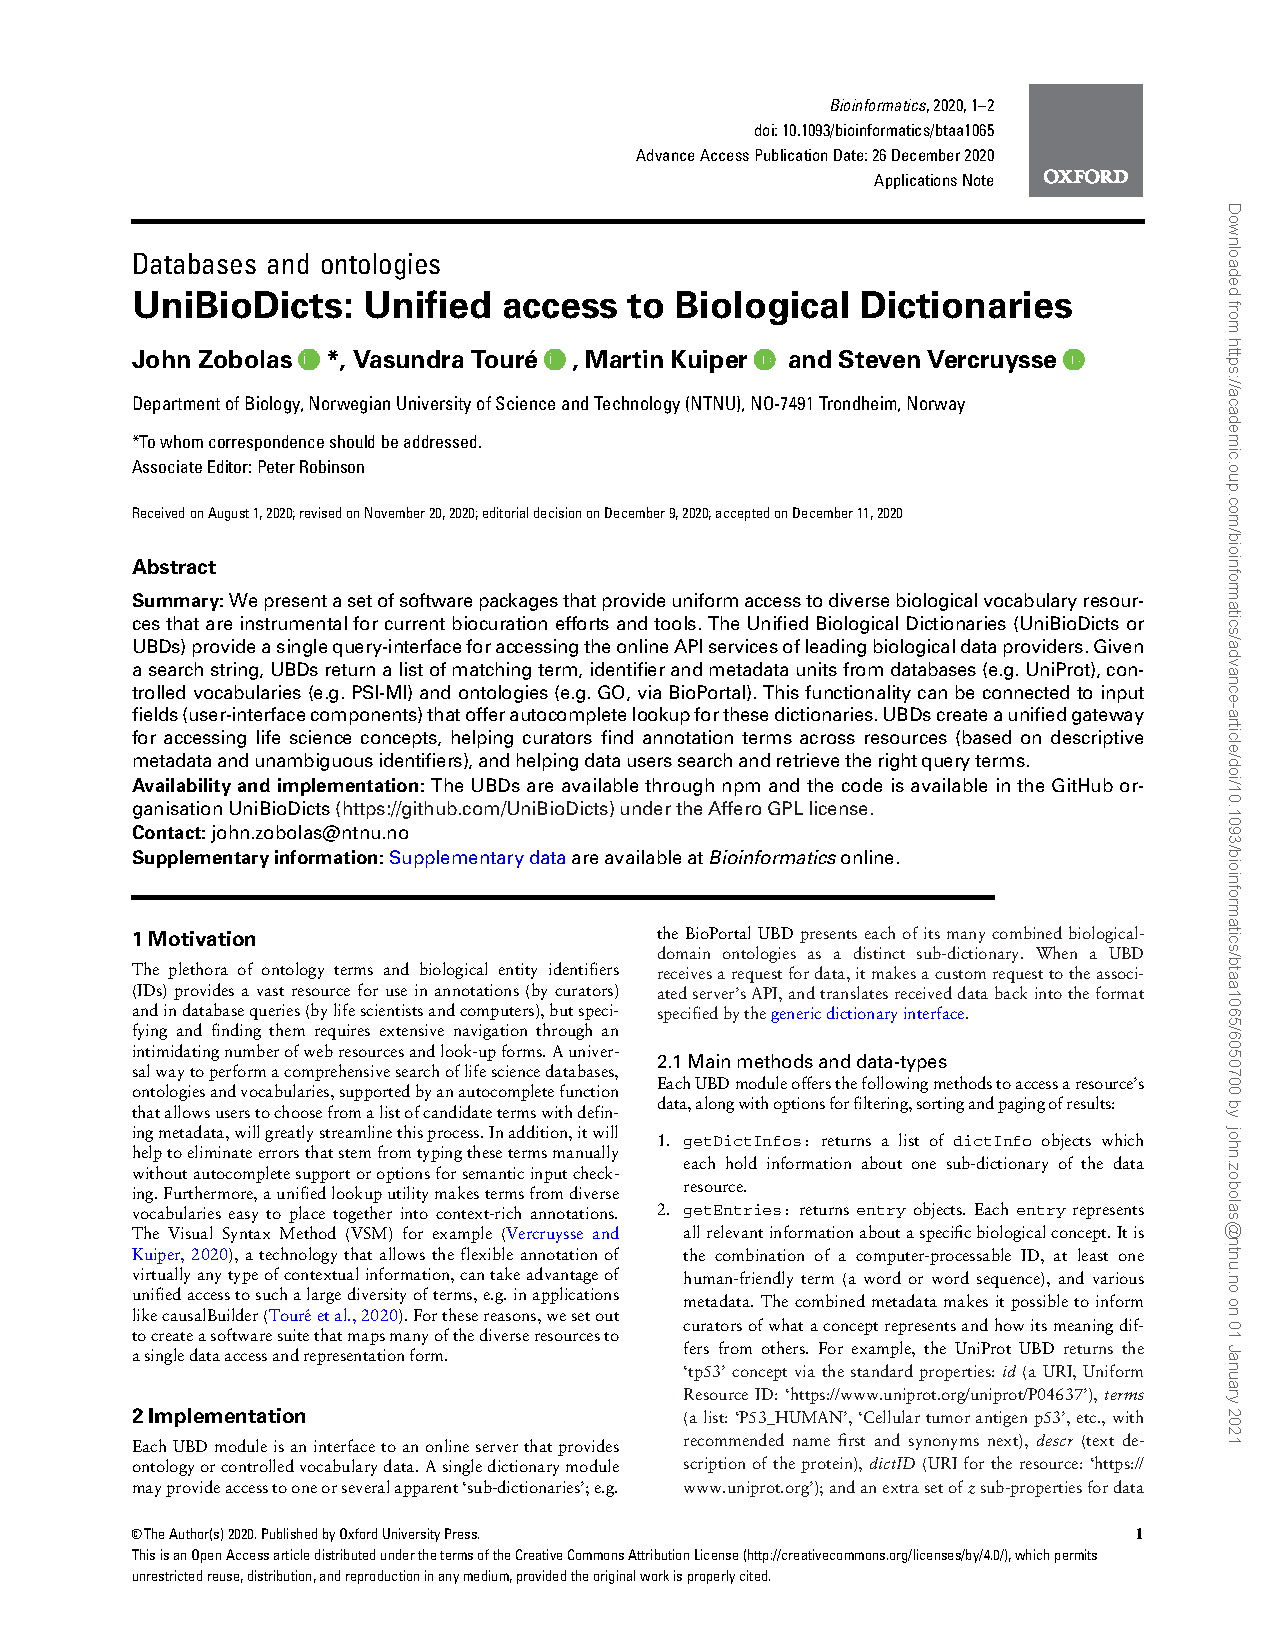
\includepdf[pages=-]{papers/ubds.pdf}
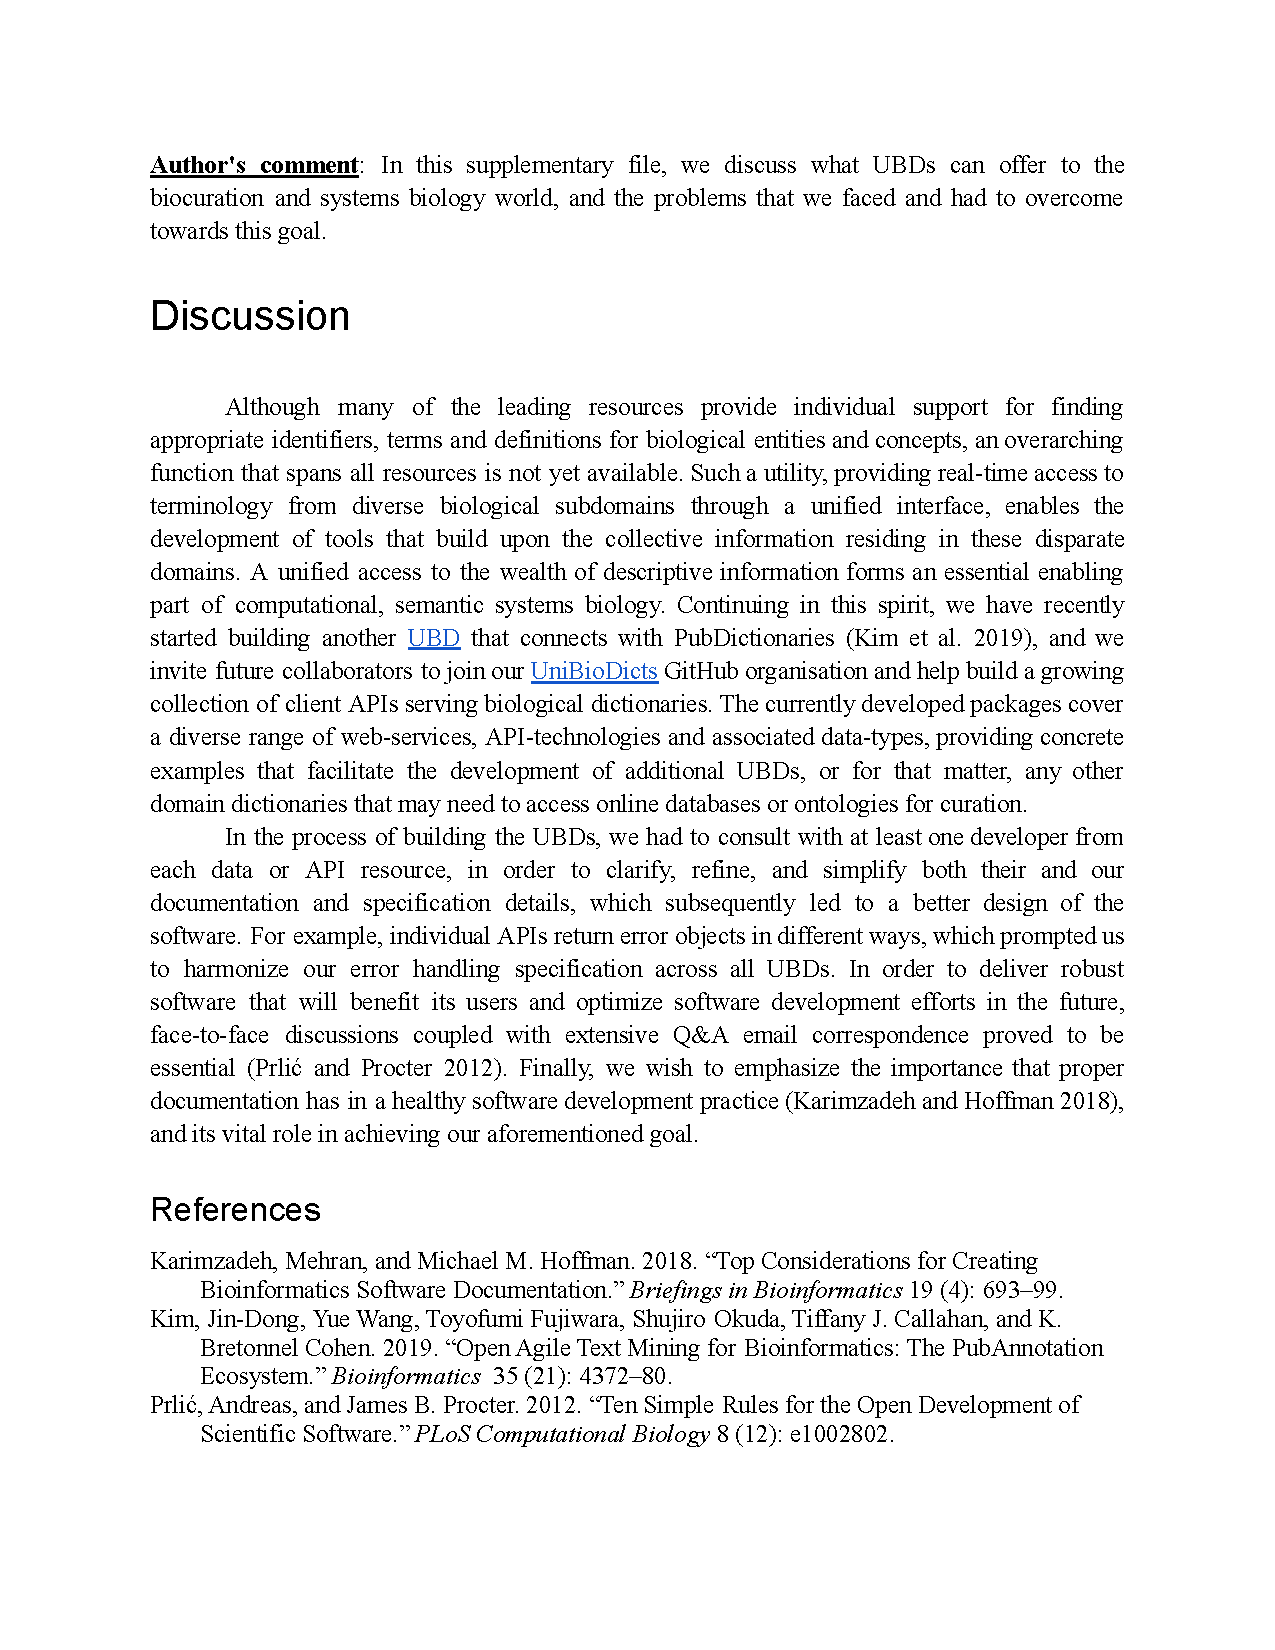
\includepdf[pages=-]{papers/ubds_supp.pdf}

\begin{center}
\vspace*{\stretch{1}}
\textbf{\fontsize{70}{1} \selectfont PAPER 2}
\vspace*{\stretch{1}}
\end{center}

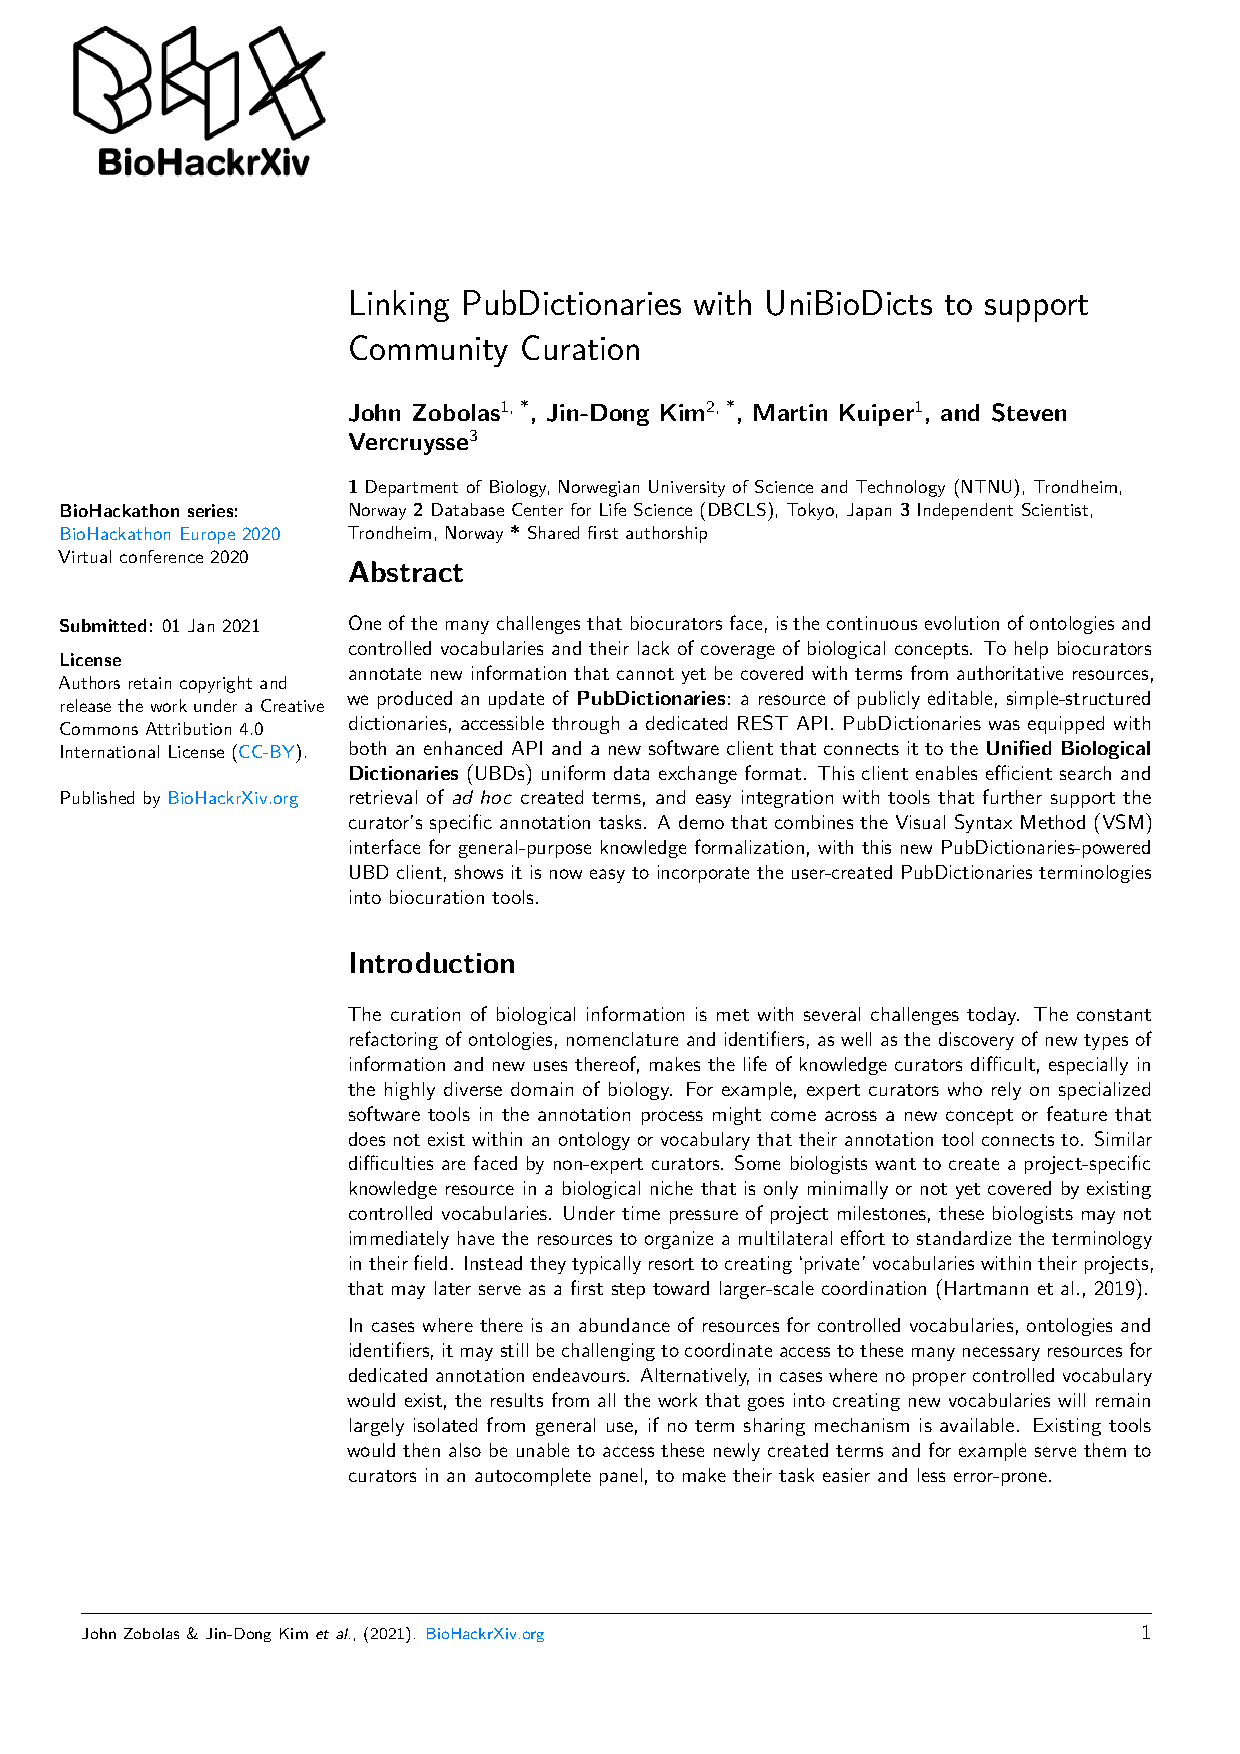
\includepdf[pages=-]{papers/pubdictionaries.pdf}

\begin{center}
\vspace*{\stretch{1}}
\textbf{\fontsize{70}{1} \selectfont PAPER 3}
\vspace*{\stretch{1}}
\end{center}

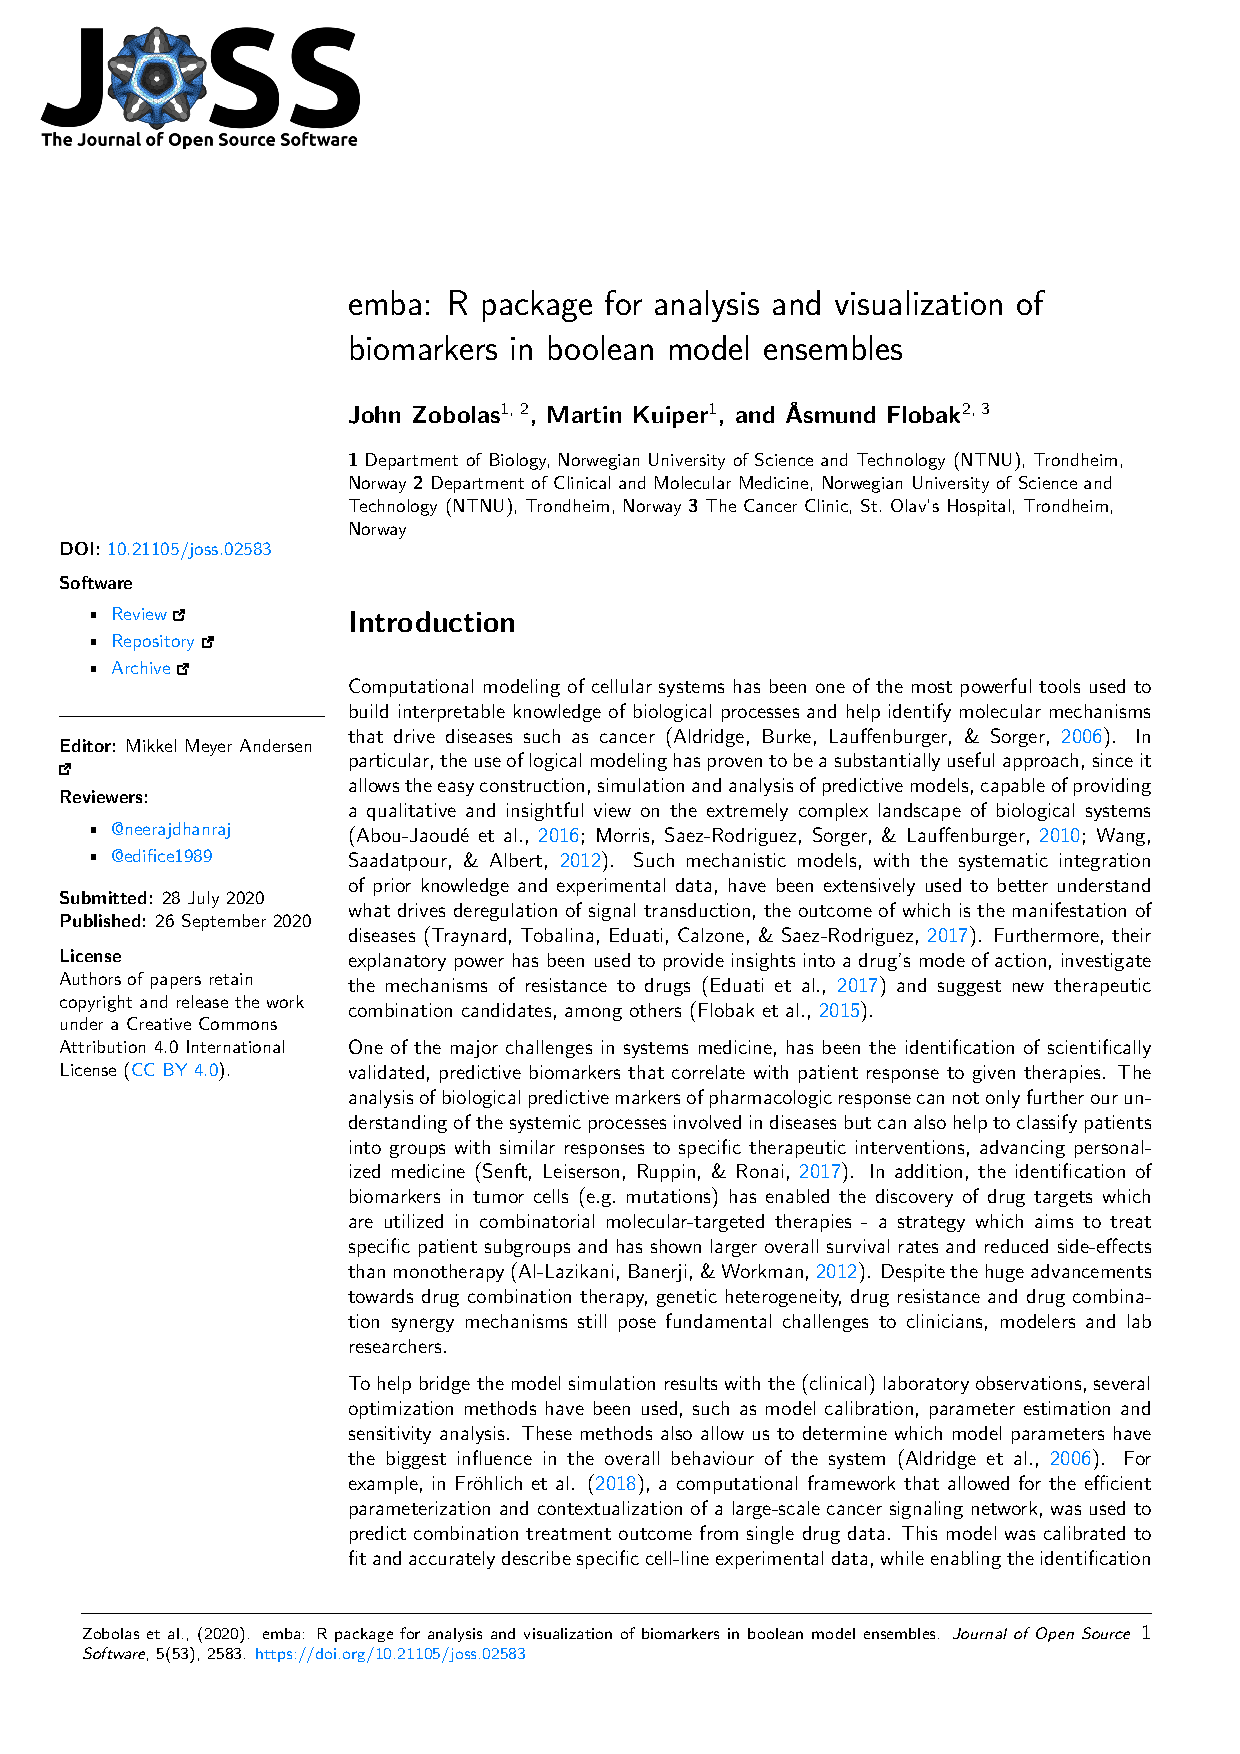
\includepdf[pages=-]{papers/emba.pdf}

\begin{center}
\vspace*{\stretch{1}}
\textbf{\fontsize{70}{1} \selectfont PAPER 4}
\vspace*{\stretch{1}}
\end{center}

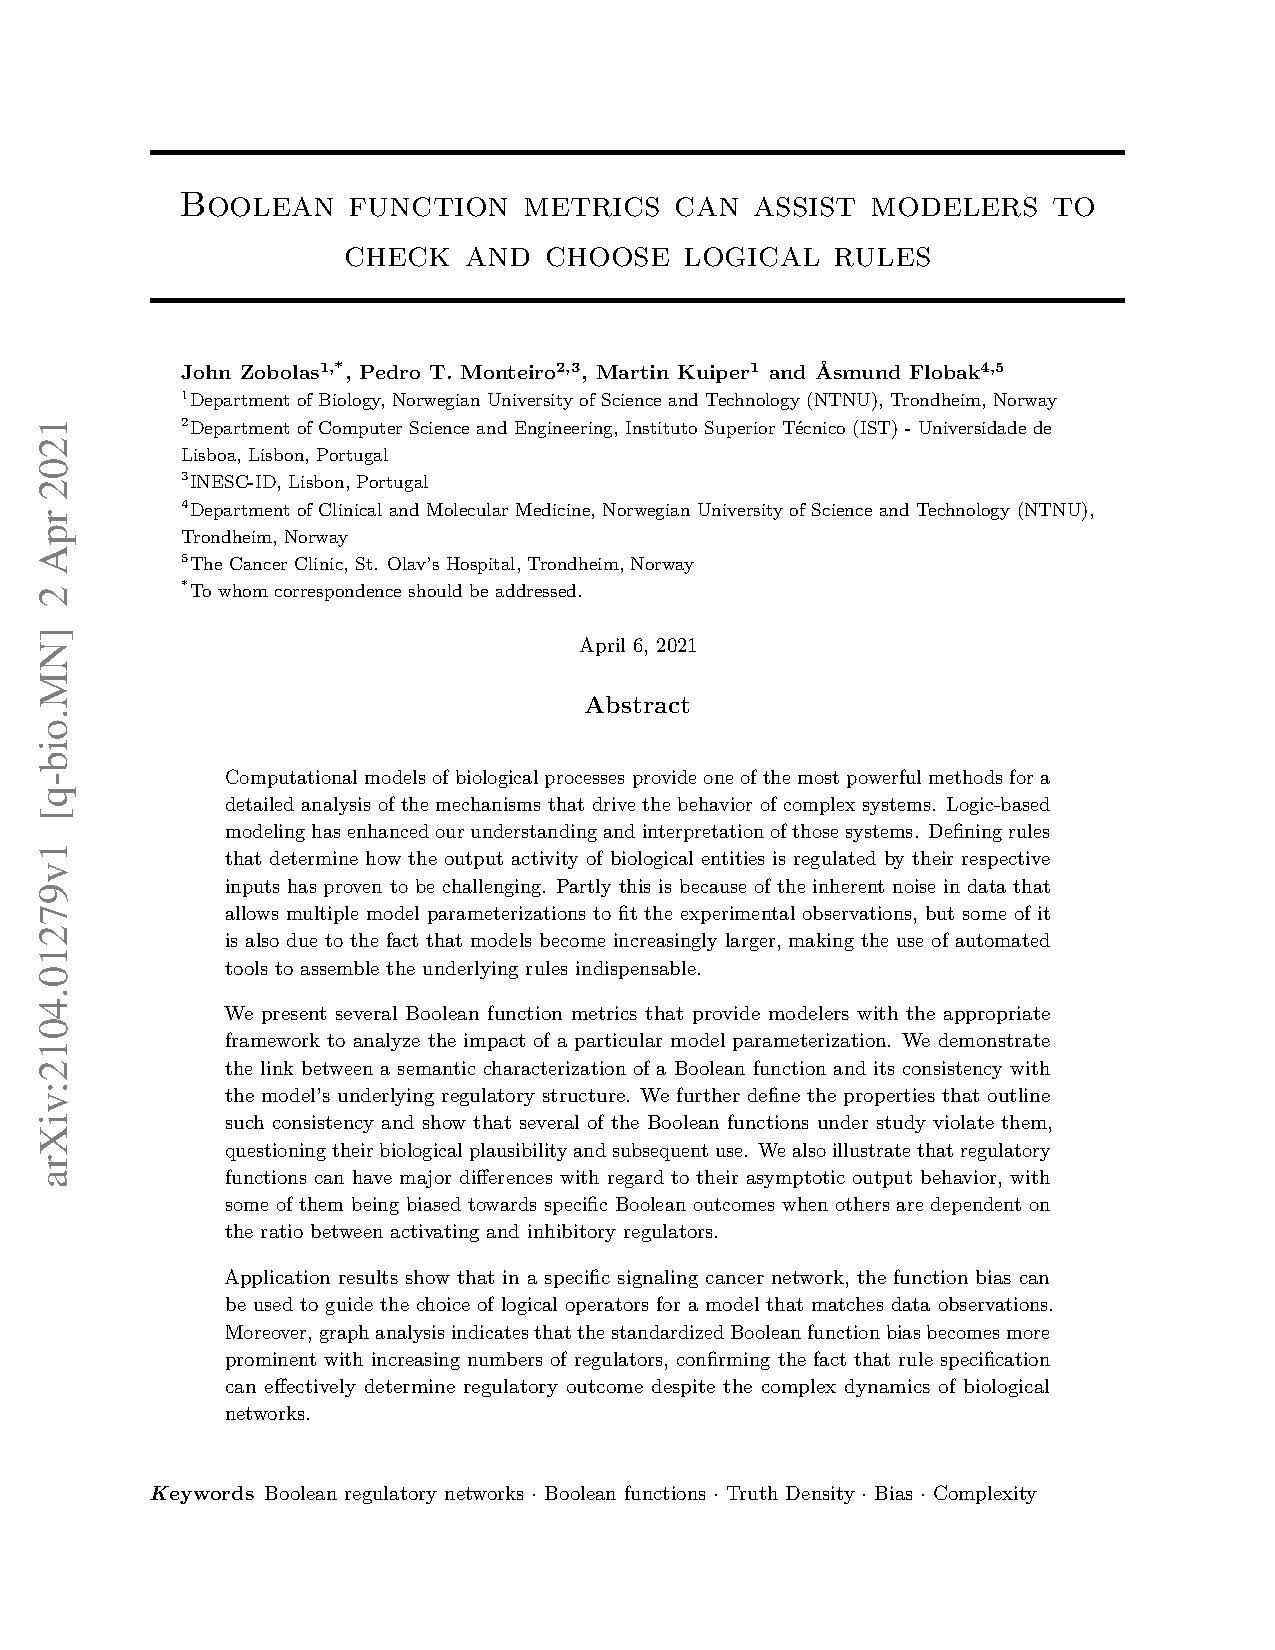
\includepdf[pages=-]{papers/bias.pdf}

\centering{-- End of Thesis --}

% list of other candidates at NTNU
%\includepdf[pages=-]{dr_ntnu.pdf}

\end{document}
